\documentclass[11pt,a4paper]{article}

% ---------- Core encoding / fonts ----------
\usepackage[utf8]{inputenc}
\usepackage[T1]{fontenc}
\usepackage{placeins}
\usepackage{lmodern}
\usepackage{microtype}
\usepackage{amssymb}

% ---------- Layout ----------
\usepackage[a4paper,left=2.6cm,right=2.6cm,top=3.4cm,bottom=3.2cm,
            headheight=14pt,headsep=22pt,footskip=28pt]{geometry}
\usepackage{tikz}
\usetikzlibrary{calc,arrows.meta,positioning,shapes.geometric,fit,backgrounds,shadows}
\usepackage{rotating}
\usepackage{pgfplots}
\pgfplotsset{compat=1.18}
\usepackage{forest}
\usepackage{eso-pic}
\usepackage{fancyhdr}
\usepackage{titlesec}
\usepackage{enumitem}
\usepackage{listings}
\usepackage{xcolor}
\lstset{
  basicstyle=\ttfamily\scriptsize,
  breaklines=true,
  breakatwhitespace=false,
  columns=fullflexible,
  frame=single,
  framerule=0.4pt,
  rulecolor=\color{black},
  backgroundcolor=\color{white},
  showstringspaces=false,
  xleftmargin=1pt,
  xrightmargin=1pt,
  tabsize=2,
  aboveskip=0.8em,
  belowskip=0.8em
}
\usepackage{hyperref}
\usepackage{parskip}
\usepackage{seqsplit}
\usepackage{booktabs}
\usepackage{array}
\usepackage{longtable}
\usepackage[most]{tcolorbox}
\usepackage{graphicx}
\usepackage{tocloft}
\usepackage[strings]{underscore}   % literal underscores in text mode, no manual escaping

% ---------- Strictly black & white ----------
\hypersetup{
  colorlinks=true,
  linkcolor=black,
  citecolor=black,
  urlcolor=black,
  pdftitle={Out-of-Band Attestation Node (OAN) -- Kernel Borderlands},
  pdfauthor={Kernel Borderlands Team}
}

% ---------- Four-side page border on every page ----------
\newcommand{\pageborder}{%
  \begin{tikzpicture}[remember picture, overlay]
    \draw[black, line width=0.7pt]
      ($(current page.north west)+(1.0cm,-1.0cm)$) rectangle
      ($(current page.south east)+(-1.0cm,1.0cm)$);
  \end{tikzpicture}%
}
\AddToShipoutPictureBG{\pageborder}

% ---------- Headers / footers ----------
\pagestyle{fancy}
\fancyhf{}
\renewcommand{\headrulewidth}{0.4pt}
\renewcommand{\footrulewidth}{0pt}
\fancyhead[L]{\small\scshape Kernel Borderlands}
\fancyhead[R]{\small\scshape Out-of-Band Attestation Node}
\fancyfoot[C]{\small\thepage}

\fancypagestyle{plain}{%
  \fancyhf{}
  \renewcommand{\headrulewidth}{0pt}
  \fancyfoot[C]{\small\thepage}
}

% ---------- Section styling ----------
\titleformat{\section}
  {\normalfont\Large\bfseries}{\thesection}{0.8em}{}
\titleformat{\subsection}
  {\normalfont\large\bfseries}{\thesubsection}{0.7em}{}
\titleformat{\subsubsection}
  {\normalfont\normalsize\bfseries\scshape}{\thesubsubsection}{0.6em}{}
\titlespacing*{\subsection}{0pt}{1.4em}{0.6em}
\titlespacing*{\subsubsection}{0pt}{1.1em}{0.4em}

\setlist[itemize]{leftmargin=1.4em, itemsep=0.2em}
\setlist[enumerate]{leftmargin=1.6em, itemsep=0.2em}

% ---------- Recurring pedagogical boxes ----------
\newtcolorbox{plainbox}{%
  colback=gray!5, colframe=black, boxrule=0.6pt, arc=1pt,
  left=8pt, right=8pt, top=6pt, bottom=6pt,
  before skip=0.9em, after skip=0.9em,
  fonttitle=\bfseries\scshape\small, title=In Plain Terms
}
\newtcolorbox{analogybox}{%
  colback=white, colframe=black!70, boxrule=0.5pt, arc=1pt,
  left=8pt, right=8pt, top=6pt, bottom=6pt,
  before skip=0.9em, after skip=0.9em,
  fonttitle=\bfseries\scshape\small, title=Analogy,
  borderline west={2pt}{0pt}{black}
}
\newtcolorbox{notebox}[1][Note]{%
  colback=gray!3, colframe=black!80, boxrule=0.5pt, arc=0pt,
  left=8pt, right=8pt, top=5pt, bottom=5pt,
  before skip=0.8em, after skip=0.8em,
  fonttitle=\bfseries\small, title={#1}
}
\newtcolorbox{statusbox}{%
  colback=white, colframe=black, boxrule=0.9pt, arc=0pt,
  left=10pt, right=10pt, top=8pt, bottom=8pt,
  before skip=1em, after skip=1em
}

% ---------- TikZ styles used across every diagram ----------
\tikzset{
  block/.style={draw=black, thick, rounded corners=2pt, align=center, fill=white,
    minimum height=0.85cm, inner sep=4pt, font=\footnotesize},
  hostblock/.style={block, fill=gray!8},
  oanblock/.style={block, fill=gray!17},
  chip/.style={block, fill=gray!22, minimum width=2.6cm, minimum height=1.1cm},
  small/.style={block, minimum height=0.6cm, font=\scriptsize},
  arr/.style={-{Latex[length=2.2mm,width=1.6mm]}, thick},
  darr/.style={-{Latex[length=2.2mm,width=1.6mm]}, thick, dashed},
  lifeline/.style={draw=black!55, thin},
  actor/.style={draw=black, thick, fill=gray!12, minimum width=2.1cm,
    minimum height=0.7cm, align=center, font=\scriptsize},
  groupbox/.style={draw=black!70, dashed, rounded corners=2pt}
}

\newcommand{\figcap}[1]{\caption{#1}}

\begin{document}

% ================= TITLE PAGE =================
\begin{titlepage}
\thispagestyle{empty}
\centering
\vspace*{\fill}

{\small\textls[280]{KERNEL BORDERLANDS}}

\vspace{1.6cm}

{\fontsize{34}{40}\selectfont\bfseries Out-of-Band\\[0.15em] Attestation Node}

\vspace{0.6em}

{\Large\bfseries OAN}

\vspace{0.9em}

{\normalsize A Hardware-Rooted Trust Anchor for Kernel Borderlands, Explained From First Principles}

\vspace{1.2cm}

{\small Design Concept Document \textbullet\ v1.0 \textbullet\ August 2026}

\vspace*{\fill}

\begin{minipage}{0.82\linewidth}
\centering
\small
\textbf{What this document is} \\[0.3em]
A complete, illustrated walkthrough of OAN: why Kernel Borderlands needs a
piece of hardware that lives outside the machine it protects, how that
hardware is put together, how it talks to the host and to itself, how it
scales from one desk to a lab, and what it costs to build. Written so a
reader with no prior security-hardware background can follow every
diagram end to end.
\end{minipage}

\vspace{1.4cm}

{\small \scshape Kernel Borderlands Team}\\[0.9em]
\small Karthik \hspace{0.5cm}\textbullet\hspace{0.5cm} PardhuVarma \hspace{0.5cm}\textbullet\hspace{0.5cm} Tejaswini \hspace{0.5cm}\textbullet\hspace{0.5cm} Rupa

\vspace{0.9em}
{\small \url{https://github.com/pardhuvarmax/kernel-borderlands}}

\vspace{1.5cm}
\end{titlepage}

% ================= TOC =================
\tableofcontents
\thispagestyle{plain}
\clearpage

% =====================================================================
\section{What Is OAN?}
\label{sec:what-is-oan}

Kernel Borderlands (KB)~\cite{repo} protects a Linux machine from the inside: an
eBPF sensor watches the kernel at Ring 0, a Go control plane scores what
it sees, and a Rust watchdog called \texttt{kb-checker} keeps an eye on
the rest of the stack from a separate process on the same box. That
covers almost every attack. It does not cover one: what happens if the
attacker gets \emph{all the way in} --- full control of the kernel
itself, the same privilege level the sensor runs at.

The \textbf{Out-of-Band Attestation Node (OAN)} is Kernel Borderlands'
answer to that one remaining case. It is a small, physically separate
computer --- its own processor, its own memory, its own power supply,
its own wiring --- that sits next to the protected machine and asks it
one question, over and over, many times a second: \emph{``are you still
telling the truth?''} If the answer stops making sense, OAN can cut the
machine's power itself, without needing any cooperation from the
machine it is cutting off.

\begin{statusbox}
\textbf{Where OAN stands today.} OAN is a design, not yet a shipped
product --- there is no code, no wire protocol, and no dedicated
repository directory for it yet. This document is the architecture that
KB intends to build: everything described below is the design target,
laid out at the level of detail needed to start building it. Where a
number is a cost estimate rather than a fixed price, it is presented as
a range for exactly that reason.
\end{statusbox}

\begin{plainbox}
Think of Kernel Borderlands today as a very well-guarded building, with
guards standing \emph{inside} the building watching every door and
hallway. OAN is a second guard station across the street, watching the
building from outside, with its own phone line, its own lights, and its
own switch for the building's power --- so that even if every guard
inside the building is somehow tricked or overpowered, the guard across
the street still notices, and can still act.
\end{plainbox}

The rest of this document builds that picture up piece by piece: why
the problem exists (\S\ref{sec:problem}), the four design rules OAN
follows (\S\ref{sec:philosophy}), how its hardware is laid out
(\S\ref{sec:architecture}--\S\ref{sec:tpm-relay}), how it actually
watches the host (\S\ref{sec:heartbeat}--\S\ref{sec:recovery}), how one
unit grows into a fleet (\S\ref{sec:scaling}--\S\ref{sec:fms}), and
finally what it costs to build one (\S\ref{sec:bom}--\S\ref{sec:budget}).

% =====================================================================
\section{The Problem OAN Solves}
\label{sec:problem}

\subsection{Software Watchdogs Have a Ceiling}

\texttt{kb-checker} already exists to solve a version of this problem.
Its entire job is to watch the rest of Kernel Borderlands from outside
their failure domain: it runs as its own process, it keeps zero
persistent state, it opens zero network sockets, and it leans on
operating-system primitives it trusts more than it trusts KB's own
code. That design is deliberately simple (KISS: Keep It Simple,
Stupid) so the watchdog itself stays small enough to actually verify by
reading it.

But ``outside their failure domain'' only stretches so far when
everything is still running on the \emph{same} machine. \texttt{kb-checker}
is a separate \emph{process}, not a separate \emph{computer}. It still
shares:

\begin{itemize}
  \item the same kernel, which arbitrates every socket it talks over,
  \item the same scheduler, which decides when (or whether) it gets to
    run,
  \item the same power and reset lines, which a kernel-level attacker
    ultimately also controls.
\end{itemize}

If an attacker achieves a full kernel compromise, they are operating at
the same privilege level as the eBPF sensor that is supposed to catch
them, and above the privilege level of the watchdog that is supposed to
notice. Software-only isolation on a single host has a ceiling: the
watchdog and the thing it watches share one root of trust --- the CPU
and the kernel running on it.

\begin{analogybox}
Imagine a company's internal auditor, who reports to the same CEO as
everyone they audit. Even a very honest, very independent-minded
auditor is still, structurally, inside the same organization. If the
CEO themselves is the problem, the auditor's independence has a limit
built into the org chart. OAN is what happens when you hire an
\emph{external} auditor who reports to nobody inside the building at
all.
\end{analogybox}

\subsection{Moving the Last Line of Defense Off the Host}

OAN's design goal is simple to state: move the very last line of
defense \emph{off the host entirely}. A physically separate node, with
its own compute and its own power domain, keeps attesting to the
host's integrity and keeps the ability to fence it, without depending
on that host's kernel being honest about anything. OAN does not
replace \texttt{kb-checker} --- it gives Kernel Borderlands an external
anchor point for the one failure mode no same-host component can
structurally cover alone: total kernel compromise.

This mirrors a decision Kernel Borderlands already made once, at a
different layer. The Critical Process Module (CPM) exists because
``the security platform's own components must be immune to the failure
modes they're meant to prevent'' at the \emph{authorization} layer ---
OAN applies that same principle one layer further down, at the
\emph{hardware} layer.

% =====================================================================
\section{A Worked Example: Anatomy of a Full Kernel Compromise}
\label{sec:worked-example}

Abstract descriptions of ``kernel compromise'' are easy to nod along to
and hard to actually picture. This section walks through one concrete
timeline, end to end, showing exactly where a software-only stack runs
out of road, and exactly where OAN picks up.

\subsection{The Scenario}

An attacker has found and exploited a memory-safety bug in a
third-party kernel module loaded on the protected host. The exploit
gives them arbitrary code execution at Ring 0 --- the same privilege
level \texttt{kb-core}'s own eBPF sensors run at. From this point on,
the attacker is not ``a process being watched by the kernel''; they
\emph{are} the kernel, in every way that matters to software running on
top of it.

\begin{figure}[h!]
\centering
\resizebox{\linewidth}{!}{%
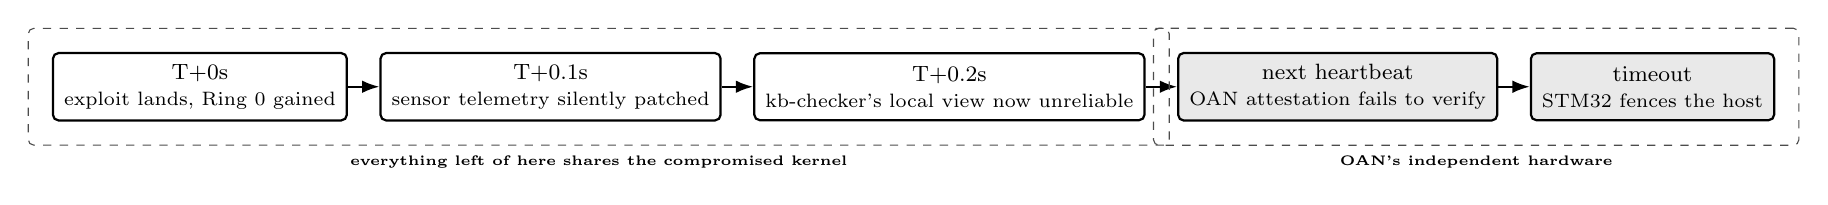
\begin{tikzpicture}[font=\scriptsize, node distance=0.42cm and 0.4cm]
  \node[block, minimum width=2.6cm] (t0) {T+0s\\\scriptsize exploit lands, Ring 0 gained};
  \node[block, right=of t0, minimum width=2.9cm] (t1) {T+0.1s\\\scriptsize sensor telemetry silently patched};
  \node[block, right=of t1, minimum width=2.9cm] (t2) {T+0.2s\\\scriptsize kb-checker's local view now unreliable};
  \node[oanblock, right=of t2, minimum width=3.1cm] (t3) {next heartbeat\\\scriptsize OAN attestation fails to verify};
  \node[oanblock, right=of t3, minimum width=2.6cm] (t4) {timeout\\\scriptsize STM32 fences the host};

  \draw[arr] (t0) -- (t1);
  \draw[arr] (t1) -- (t2);
  \draw[arr] (t2) -- (t3);
  \draw[arr] (t3) -- (t4);

  \node[groupbox, fit=(t0)(t1)(t2), inner sep=0.3cm, label={[font=\tiny\bfseries]below:everything left of here shares the compromised kernel}] (left) {};
  \node[groupbox, fit=(t3)(t4), inner sep=0.3cm, label={[font=\tiny\bfseries]below:OAN's independent hardware}] (right) {};
\end{tikzpicture}%
}
\figcap{The same timeline, seen from two different trust domains. The left three boxes all run on the compromised kernel; the right two never do.}
\label{fig:timeline}
\end{figure}

\subsection{Minute Zero: What the Attacker Can Reach}

Once Ring 0 is theirs, the attacker can, in principle, do all of the
following without any of it looking unusual from inside the host:

\begin{itemize}
  \item Patch the eBPF sensor's own view of the syscall table, so
    \texttt{kb-core} keeps reporting a clean process tree.
  \item Starve or suspend the \texttt{kb-checker} process at the
    scheduler level, so it never gets CPU time to notice anything is
    wrong.
  \item Forge normal-looking heartbeats on any socket the kernel itself
    arbitrates --- because the kernel arbitrates all of them.
  \item Leave the host's power and reset lines exactly as they were, so
    nothing about the machine's outward behavior changes.
\end{itemize}

\begin{plainbox}
This is the precise moment every \emph{purely software} defense runs out
of road. Every one of the bullets above is a case of ``ask the kernel
whether the kernel is honest'' --- and a fully compromised kernel will
always answer yes. There is no cleverer question you can ask it in
software that gets around this, because software questions all have to
travel through the same compromised kernel to get an answer.
\end{plainbox}

\subsection{Where OAN Picks Up}

None of the four bullets above touch OAN, for a simple structural
reason: OAN never asked the kernel a question that the kernel could
answer on the attacker's behalf in the first place.

\begin{enumerate}
  \item \textbf{The next heartbeat is due.} \texttt{kb-checker}'s
    attestation either does not arrive on the OOB link at all (because
    the process was starved), or arrives but fails TPM verification
    (because the sealed measurements no longer match).
  \item \textbf{The SBC does not reset the STM32's liveness timer.} It
    only ever does this after a valid, verified attestation --- and
    there is not one.
  \item \textbf{The STM32's own clock, running independently of
    anything on the host or the SBC, reaches the configured timeout.}
  \item \textbf{The fail-closed policy fires.} The relay --- wired
    directly to the STM32, never to the SBC or the host --- cuts power
    or reset, physically, regardless of what the compromised kernel is
    doing or reporting at that instant.
\end{enumerate}

The attacker's Ring 0 access, which was total with respect to the host,
grants them precisely nothing with respect to the STM32's timer or the
relay it drives --- those never took input from the host to begin with.
That gap is the entire reason OAN exists.

% =====================================================================
\section{Design Philosophy}
\label{sec:philosophy}

Everything about OAN follows from four rules. They deliberately mirror
\texttt{kb-checker}'s own KISS pillars, moved from the software layer to
the hardware layer.

\begin{center}
\renewcommand{\arraystretch}{1.35}
\begin{tabular}{@{}p{3.1cm}p{10.6cm}@{}}
\toprule
\textbf{Principle} & \textbf{What it means in practice} \\
\midrule
Out-of-Band & OAN never depends on the monitored operating system for
its own execution. It has its own boot chain, its own clock, its own
storage. \\
Independent & Own CPU, own memory, own storage, own power. No shared
failure domain with the host --- if the host's power supply dies,
loses network, or is compromised, none of that touches OAN. \\
Hardware-Rooted & Trust originates from a physical chip (a TPM 2.0
module), not from a software claim that could itself be forged by a
compromised kernel. \\
Fail-Safe (configurable) & OAN can take protective action even when
the host cannot cooperate. The exact failure behavior --- fence
immediately, or leave the host running and only alert --- is a
deployment-level policy switch, described in \S\ref{sec:heartbeat},
defaulting to the safer of the two. \\
\bottomrule
\end{tabular}
\end{center}

Read together, these four rules answer the same question from four
different angles: \emph{``what happens to OAN's trustworthiness if the
host is fully owned by an attacker?''} The answer, by design, is
nothing --- OAN keeps working exactly as before, because nothing about
its own operation ever routed through the host in the first place.

% =====================================================================
\section{High-Level Architecture}
\label{sec:architecture}

At the top level, OAN sits beside the existing Kernel Borderlands host
and talks to exactly one of its five subsystems directly:
\texttt{kb-checker}. It never talks to \texttt{kb-core} or
\texttt{kb-control-plane} directly, because \texttt{kb-checker} is
already the one KB component whose entire purpose is external
verification --- it is the natural point of contact on the host side.

\begin{figure}[h!]
\centering
\resizebox{\linewidth}{!}{%
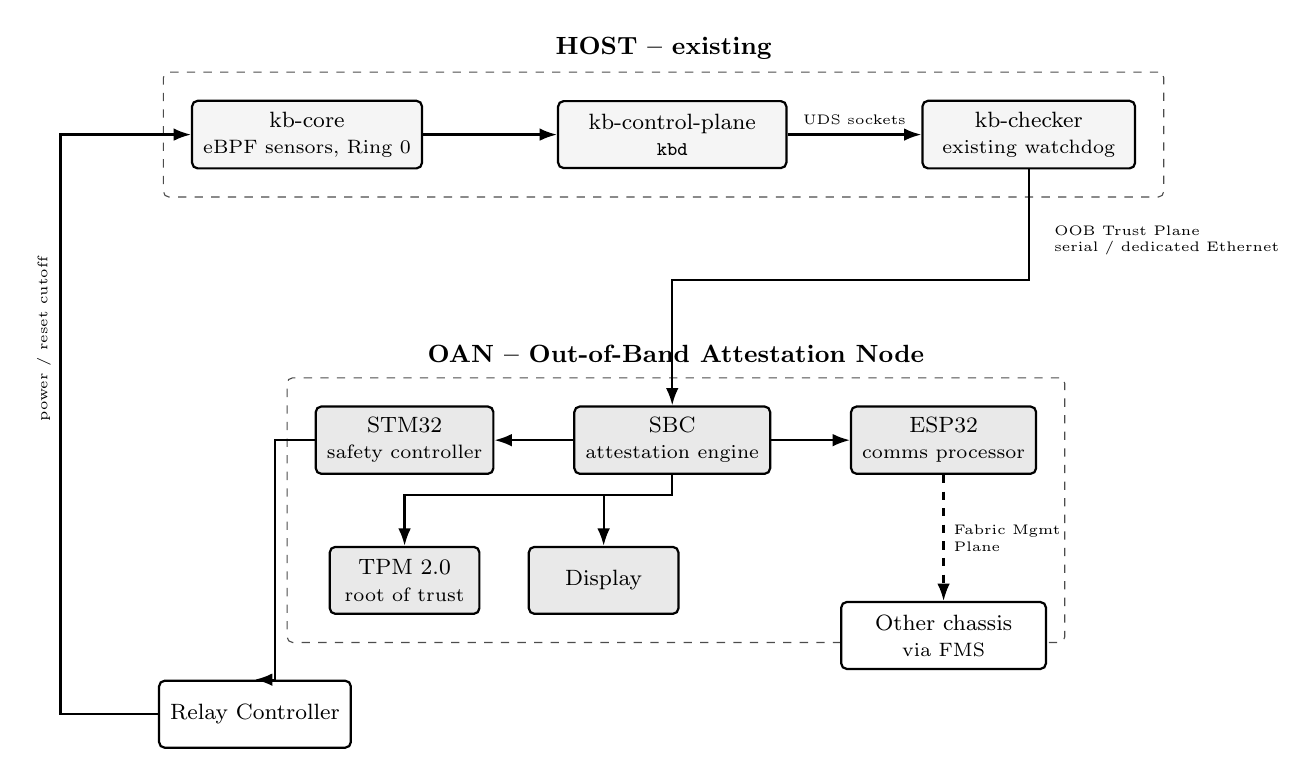
\begin{tikzpicture}[node distance=0.6cm and 1.7cm, font=\footnotesize]

  % HOST row -- wide gaps so inline arrow labels always have room
  \node[hostblock, minimum width=2.6cm] (core) {kb-core\\\scriptsize eBPF sensors, Ring 0};
  \node[hostblock, right=of core, minimum width=2.9cm] (cp) {kb-control-plane\\\scriptsize \texttt{kbd}};
  \node[hostblock, right=of cp, minimum width=2.7cm] (kbc) {kb-checker\\\scriptsize existing watchdog};

  \draw[arr] (core.east) -- (cp.west);
  \draw[arr] (cp.east) -- (kbc.west) node[midway, above, font=\tiny]{UDS sockets};

  \node[groupbox, fit=(core)(cp)(kbc), inner sep=0.35cm] (hostbox) {};
  \node[font=\small\bfseries] at ($(hostbox.north)+(0,0.3)$) {HOST -- existing};

  % OAN row 1: STM32 - SBC - ESP32
  \node[oanblock, below=3.0cm of cp, minimum width=2.4cm] (sbc) {SBC\\\scriptsize attestation engine};
  \node[oanblock, left=1.0cm of sbc, minimum width=1.9cm] (stm) {STM32\\\scriptsize safety controller};
  \node[oanblock, right=1.0cm of sbc, minimum width=1.9cm] (esp) {ESP32\\\scriptsize comms processor};

  % OAN row 2: TPM - Display, below row 1
  \node[oanblock, below=0.9cm of stm, minimum width=1.9cm] (tpm) {TPM 2.0\\\scriptsize root of trust};
  \node[oanblock, right=0.6cm of tpm, minimum width=1.9cm] (disp) {Display};

  \draw[arr] (sbc) -- (stm);
  \draw[arr] (sbc) -- (esp);
  \draw[arr] (sbc.south) -- ++(0,-0.25) -| (tpm.north);
  \draw[arr] (sbc.south) -- ++(0,-0.25) -| (disp.north);

  \node[groupbox, fit=(stm)(sbc)(esp)(tpm)(disp), inner sep=0.35cm] (oanbox) {};
  \node[font=\small\bfseries] at ($(oanbox.north)+(0,0.3)$) {OAN -- Out-of-Band Attestation Node};

  % OOB Trust Plane: kb-checker straight down to SBC's row height, then left into SBC
  \draw[arr] (kbc.south) -- ++(0,-1.4) -| (sbc.north);
  \node[font=\tiny, align=left, anchor=west] at ($(kbc.south)+(0.2,-0.9)$)
    {OOB Trust Plane\\serial / dedicated Ethernet};

  % Relay path: STM32 out to the left, then down to Relay -- never drops
  % straight through the TPM/Display row below it; Relay back up to
  % kb-core, routed along a dedicated coordinate far to the left of every box
  \node[block, below=2.6cm of stm, xshift=-1.9cm, minimum width=2.1cm] (relay) {Relay Controller};
  \draw[arr] (stm.west) -- ++(-0.5,0) |- (relay.north);

  \coordinate (leftrail) at ($(hostbox.west)+(-1.3,0)$);
  \draw[arr] (relay.west) -| (leftrail) |- (core.west);
  \node[font=\tiny, align=center, rotate=90, anchor=south] at ($(leftrail)+(0,-2.6)$)
    {power / reset cutoff};

  % Fabric Management Plane, directly below ESP32 -- simple straight arrow
  \node[block, below=1.6cm of esp, minimum width=2.6cm] (fms) {Other chassis\\\scriptsize via FMS};
  \draw[darr] (esp.south) -- (fms.north)
    node[midway, right, font=\tiny, align=left]{Fabric Mgmt\\Plane};

\end{tikzpicture}%
}
\figcap{OAN sits beside the host, talking only to \texttt{kb-checker} over a dedicated out-of-band link. The relay gives OAN a physical, software-independent way to cut the host's power.}
\label{fig:architecture}
\end{figure}

Three things in Figure~\ref{fig:architecture} carry the whole design:

\begin{itemize}
  \item \textbf{The OOB link is not the host's network.} It is a
    dedicated serial line or a dedicated Ethernet port that never
    touches the host's normal network stack, so a compromised host
    cannot reach it the way it could reach a regular NIC.
  \item \textbf{The relay is driven by the STM32, not the SBC.} Fencing
    survives a full Linux crash on OAN's own SBC, because the chip that
    controls the relay never runs Linux at all (\S\ref{sec:stm32}).
  \item \textbf{Fleet traffic is a separate, dashed line.} Anything
    that talks to other chassis goes out through the ESP32 on a
    completely different physical channel (\S\ref{sec:planes}).
\end{itemize}

% =====================================================================
\section{Two Communication Planes}
\label{sec:planes}

OAN exposes two communication channels that never share a wire, a
switch, or a protocol stack. Keeping them apart is what lets OAN scale
to a fleet (\S\ref{sec:scaling}) without ever weakening the one link
that actually matters for trust.

\begin{figure}[h!]
\centering
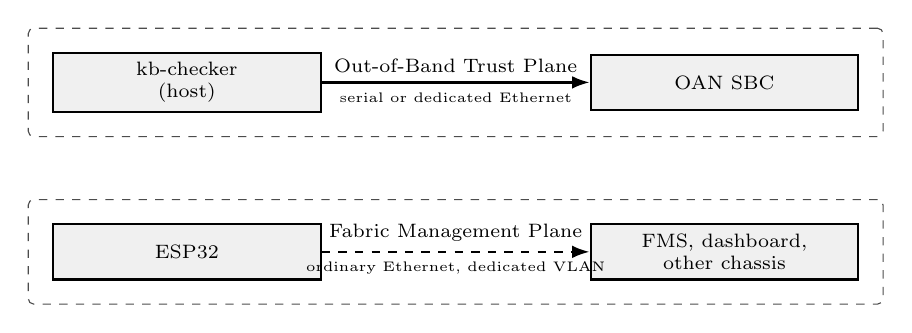
\begin{tikzpicture}[font=\footnotesize, node distance=1.1cm]
  \node[actor, minimum width=3.4cm] (kbc) {kb-checker\\\scriptsize (host)};
  \node[actor, right=3.4cm of kbc, minimum width=3.4cm] (sbc) {OAN SBC};
  \draw[arr] (kbc) -- node[above, font=\scriptsize]{Out-of-Band Trust Plane} node[below, font=\tiny]{serial or dedicated Ethernet} (sbc);

  \node[below=1.4cm of kbc, actor, minimum width=3.4cm] (esp) {ESP32};
  \node[right=3.4cm of esp, actor, minimum width=3.4cm] (fms) {FMS, dashboard,\\other chassis};
  \draw[darr] (esp) -- node[above, font=\scriptsize]{Fabric Management Plane} node[below, font=\tiny]{ordinary Ethernet, dedicated VLAN} (fms);

  \node[groupbox, fit=(kbc)(sbc), inner sep=0.3cm] (t1) {};
  \node[groupbox, fit=(esp)(fms), inner sep=0.3cm] (t2) {};
\end{tikzpicture}
\figcap{Two planes, two purposes. The top plane establishes trust; the bottom plane only coordinates a fleet that already trusts itself locally.}
\label{fig:planes}
\end{figure}

\begin{center}
\renewcommand{\arraystretch}{1.3}
\begin{tabular}{@{}p{3.6cm}p{4.9cm}p{4.9cm}@{}}
\toprule
 & \textbf{OOB Trust Plane} & \textbf{Fabric Management Plane} \\
\midrule
Carries & Attestation, heartbeat, recovery/fencing triggers & Fleet discovery, policy sync, dashboards, event aggregation \\
Owner chip & SBC (direct link) & ESP32 \\
Shared between hosts? & Never --- physical, point-to-point per host & Yes --- ordinary networking across the fleet \\
Required for basic protection? & Yes --- this \emph{is} the trust boundary & No --- see the Local Autonomy Principle, \S\ref{sec:autonomy} \\
\bottomrule
\end{tabular}
\end{center}

\begin{plainbox}
The Fabric Management Plane is allowed to be ``just Ethernet'' precisely
because it never carries anything security-critical. It only ever sees
signed summaries that OAN's own trust plane has already vouched for
(\S\ref{sec:fms}) --- so even a fully compromised management network
can't forge a clean bill of health for a host that is actually
compromised.
\end{plainbox}

% =====================================================================
\section{Meet the Three Processors}
\label{sec:three-chips}

OAN's brain is deliberately split across three separate chips, each
with exactly one job. The split looks like extra hardware at first
glance, but it is the single most important decision in the whole
design: it means no one chip is ever both ``the thing that makes the
security decision'' and ``the thing that runs a full general-purpose,
network-facing operating system.''

\begin{figure}[h!]
\centering
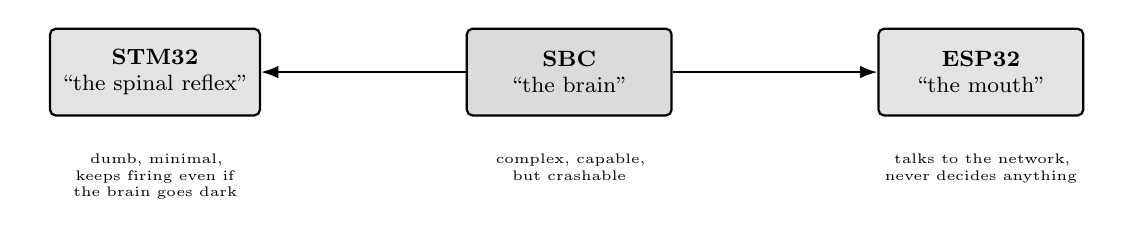
\begin{tikzpicture}[font=\scriptsize, node distance=1.6cm]
  \node[chip, fill=gray!28] (sbc) {\bfseries SBC\\``the brain''};
  \node[chip, left=2.6cm of sbc] (stm) {\bfseries STM32\\``the spinal reflex''};
  \node[chip, right=2.6cm of sbc] (esp) {\bfseries ESP32\\``the mouth''};

  \draw[arr] (sbc) -- (stm);
  \draw[arr] (sbc) -- (esp);

  \node[below=0.35cm of sbc, font=\tiny, align=center, text width=3.4cm] {complex, capable,\\but crashable};
  \node[below=0.35cm of stm, font=\tiny, align=center, text width=3.0cm] {dumb, minimal,\\keeps firing even if\\the brain goes dark};
  \node[below=0.35cm of esp, font=\tiny, align=center, text width=3.0cm] {talks to the network,\\never decides anything};
\end{tikzpicture}
\figcap{The three-chip split, in one picture. Each chip is deliberately worse at the other two chips' jobs than it is at its own.}
\label{fig:threechips}
\end{figure}

\subsection{SBC --- The Brain}
\label{sec:sbc}

The SBC (a small board like a Raspberry Pi, or an Intel N100 mini PC for
the shared-chassis design, \S\ref{sec:scaling}) is the counterpart to
\texttt{kb-checker}'s role, but running on independent hardware. It
carries:

\begin{itemize}
  \item the main attestation engine and policy engine,
  \item cluster management (the Fabric Management Service,
    \S\ref{sec:fms}),
  \item the local dashboard and database,
  \item cryptographic verification of everything the host reports,
  \item logging.
\end{itemize}

This is the only chip in OAN complex enough to run a full Linux
userspace, and therefore the only one complex enough to have bugs, hang,
or crash. Everything downstream of it is built assuming exactly that
will eventually happen.

\subsection{STM32 --- The Spinal Reflex}
\label{sec:stm32}

The STM32 is a tiny microcontroller with one job: watch a timer, and
flip a relay if the timer runs out. It has no operating system, no
network stack, and no scheduler --- just one small, deterministic
firmware loop.

\begin{itemize}
  \item Hardware independent watchdog timer (IWDG).
  \item Heartbeat supervision, on its own clock.
  \item Relay control and emergency fencing.
  \item Safe-state controller for the whole appliance.
\end{itemize}

\begin{analogybox}
A spinal reflex --- pulling your hand off a hot stove --- happens before
the signal even reaches your brain. It is fast precisely because it is
\emph{not} doing any complicated thinking. The STM32 is built the same
way: it is not smart enough to be tricked, because it is not smart
enough to do anything except watch a clock and flip a switch.
\end{analogybox}

\subsubsection{Why a Dedicated Chip, Not the SBC or the ESP32}

Two questions come up immediately, and both have concrete answers.

\textbf{Why not let the SBC drive the relay directly?} Because then
fencing depends on Linux being alive and scheduled promptly. If the SBC
hangs, panics, or is simply busy at the wrong moment, the fencing
decision hangs with it --- recreating, one level down, the exact
same-failure-domain problem OAN exists to solve for the host in the
first place.

\textbf{Why not use the ESP32, since it is already on the board?}
Because the ESP32 runs a full Wi-Fi and networking stack --- a much
larger, more remotely-reachable attack surface, and the chip most
likely to be running stock SDK code with known vulnerabilities. Handing
fencing authority to the least-trusted, most network-exposed chip on
the board would be exactly backwards.

The STM32 costs a few dollars precisely \emph{because} it does not do
policy or attestation logic --- that stays on the SBC. It only watches
a timer and flips a relay, a job small enough for a commodity board to
do with very high confidence, no custom safety-rated silicon required.

\subsection{ESP32 --- The Mouth}

The ESP32 is the dedicated management and communications processor. It
handles device discovery, secure provisioning, the maintenance
interface, and optional wireless management --- and it is the chip that
owns the Fabric Management Plane (\S\ref{sec:planes}).

The ESP32 never makes a security decision on its own. It only carries
traffic. That single restriction is what makes it safe for the ESP32 to
also be the chip most exposed to ordinary networking: a compromise of
the ESP32 or the management plane it carries cannot reach the
attestation or relay path at all, because that path lives entirely on
the SBC/STM32/TPM side of the board.

% =====================================================================
\section{TPM 2.0 and the Relay: Trust and Fencing}
\label{sec:tpm-relay}

\subsection{TPM 2.0 --- Hardware Root of Trust}

A Trusted Platform Module (TPM) is a small, dedicated security chip
built for exactly one purpose: storing cryptographic keys and integrity
measurements in a way that even the computer it is attached to cannot
tamper with from software alone. OAN's TPM does double duty:

\begin{itemize}
  \item \textbf{Seals OAN's own integrity state.} Measured boot on the
    SBC and STM32 firmware is sealed against the TPM, so OAN can prove
    its own software has not been tampered with --- the same property
    it is asking the host to prove about itself.
  \item \textbf{Verifies \texttt{kb-checker}'s reported state.} Each
    attestation \texttt{kb-checker} sends over the OOB link is checked
    against sealed reference measurements in the TPM, so a compromised
    host kernel cannot simply forge a clean report.
\end{itemize}

\begin{plainbox}
Sealing \emph{both} sides against the same physical chip closes a gap
that would otherwise exist: it is not enough for OAN to trust the host
--- OAN's own word has to be worth something too. A TPM that only
checked the host, sitting inside an OAN whose own integrity nobody
verified, would just move the same trust problem one hop over rather
than solving it.
\end{plainbox}

\subsection{Relay Controller --- Physical Fencing}

The relay is the final, physical link in the chain: a switch that can
cut or restore the host's power or reset line, wired directly to the
STM32 (\S\ref{sec:stm32}), never to the SBC. It is used only after
software-level recovery has already failed (\S\ref{sec:recovery}), and
its behavior on link loss is a configured policy rather than a fixed
reflex:

\begin{center}
\renewcommand{\arraystretch}{1.3}
\begin{tabular}{@{}p{3.4cm}p{10.3cm}@{}}
\toprule
\textbf{Policy} & \textbf{Behavior} \\
\midrule
Fail-closed (default) & If the OOB link drops, or an attestation is
missing or invalid past the configured timeout, the STM32 fences the
host --- favoring protection over uptime. \\
Fail-open & The host is left running and an alert is raised instead;
chosen deliberately for availability-critical hosts where an
unattended, unverified fencing event would itself be an unacceptable
outage. \\
\bottomrule
\end{tabular}
\end{center}

Fail-closed is the default because it matches the same principle the
Critical Process Module already applies elsewhere in Kernel
Borderlands: fail closed toward protection. A deployment can opt a
specific host into fail-open, but it has to do so explicitly.

\subsection{Display}

A small display (an I2C OLED or LCD panel) shows host status,
integrity state, threat level, heartbeat, cluster health, TPM status,
relay status, and a rolling event log. It is a read-only reflection of
state the SBC and STM32 already hold --- useful for a technician
standing in front of the chassis, but never an input to any decision
OAN makes.

% =====================================================================
\section{What OAN Does, Continuously}

Once running, OAN's loop never stops:

\begin{itemize}
  \item Verifies host integrity against sealed TPM measurements.
  \item Confirms \texttt{kb-checker} liveness on every heartbeat.
  \item Validates each attestation the host sends.
  \item Detects heartbeat loss and suspicious silence.
  \item Logs every security-relevant event locally.
  \item Coordinates software-level recovery before ever reaching for
    the relay.
  \item Performs last-resort hardware fencing when every other option
    is exhausted.
\end{itemize}

% =====================================================================
\section{The Attestation Heartbeat}
\label{sec:heartbeat}

Every interval, \texttt{kb-checker} on the host sends a signed
attestation across the OOB link. The SBC checks it against the TPM,
and --- if it is valid --- resets a liveness timer on the STM32. That
timer is the entire mechanism: as long as valid attestations keep
arriving on schedule, the STM32 has nothing to do. The moment they
stop, or start failing verification, the STM32's own clock takes over.

\begin{figure}[h!]
\centering
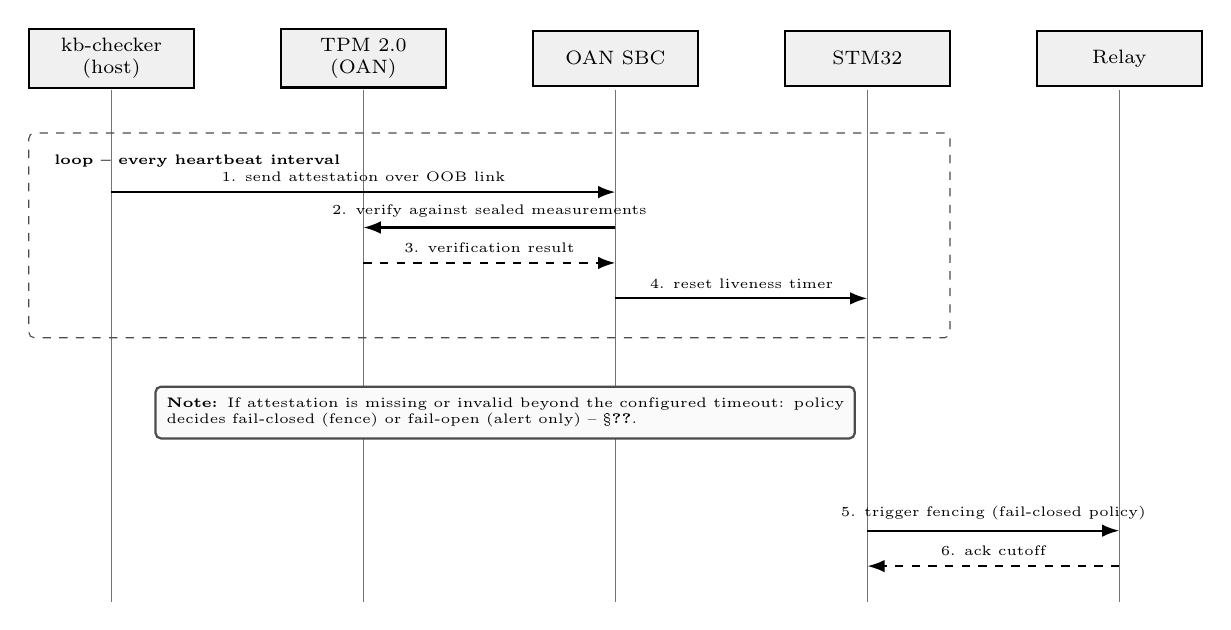
\begin{tikzpicture}[font=\scriptsize]
  \def\yTop{0}
  \def\yBot{-6.9}

  \node[actor] (kbc) at (0,\yTop) {kb-checker\\\scriptsize (host)};
  \node[actor] (tpm) at (3.2,\yTop) {TPM 2.0\\\scriptsize (OAN)};
  \node[actor] (sbc) at (6.4,\yTop) {OAN SBC};
  \node[actor] (stm) at (9.6,\yTop) {STM32};
  \node[actor] (rel) at (12.8,\yTop) {Relay};

  \foreach \x in {0,3.2,6.4,9.6,12.8}{
    \draw[lifeline] (\x,\yTop-0.4) -- (\x,\yBot);
  }

  \node[groupbox, fit={(-0.9,-1.1) (10.5,-3.4)}, inner sep=0.15cm] (loopbox) {};
  \node[font=\tiny\bfseries, anchor=west] at (-0.85,-1.3) {loop -- every heartbeat interval};

  \draw[arr] (0,-1.7) -- node[above, font=\tiny]{1. send attestation over OOB link} (6.4,-1.7);
  \draw[arr] (6.4,-2.15) -- node[above, font=\tiny]{2. verify against sealed measurements} (3.2,-2.15);
  \draw[darr] (3.2,-2.6) -- node[above, font=\tiny]{3. verification result} (6.4,-2.6);
  \draw[arr] (6.4,-3.05) -- node[above, font=\tiny]{4. reset liveness timer} (9.6,-3.05);

  \node[draw=black!70, thick, rounded corners=2pt, fill=gray!4, align=left,
    font=\tiny, text width=8.6cm, inner sep=4pt] at (5.0,-4.5)
    {\textbf{Note:} If attestation is missing or invalid beyond the
     configured timeout: policy decides fail-closed (fence) or
     fail-open (alert only) -- \S\ref{sec:heartbeat}.};

  \draw[arr] (9.6,-6.0) -- node[above, font=\tiny]{5. trigger fencing (fail-closed policy)} (12.8,-6.0);
  \draw[darr] (12.8,-6.45) -- node[above, font=\tiny]{6. ack cutoff} (9.6,-6.45);
\end{tikzpicture}
\figcap{The attestation heartbeat. Steps 1--4 repeat forever while everything is healthy; steps 5--6 only fire when the loop breaks and the fail-closed policy is active.}
\label{fig:heartbeat}
\end{figure}

\begin{plainbox}
This is why the STM32 does not need to understand cryptography at all.
It never verifies an attestation itself --- it only watches whether the
SBC \emph{keeps telling it to reset the clock}. Verification happens
once, on the SBC, where the TPM lives; the STM32's only job downstream
of that is noticing silence.
\end{plainbox}

% =====================================================================
\section{Where OAN Sits in the Trust Boundary}

Zooming out, OAN's place in the overall Kernel Borderlands data flow is
a single, sharp line:

\begin{figure}[h!]
\centering
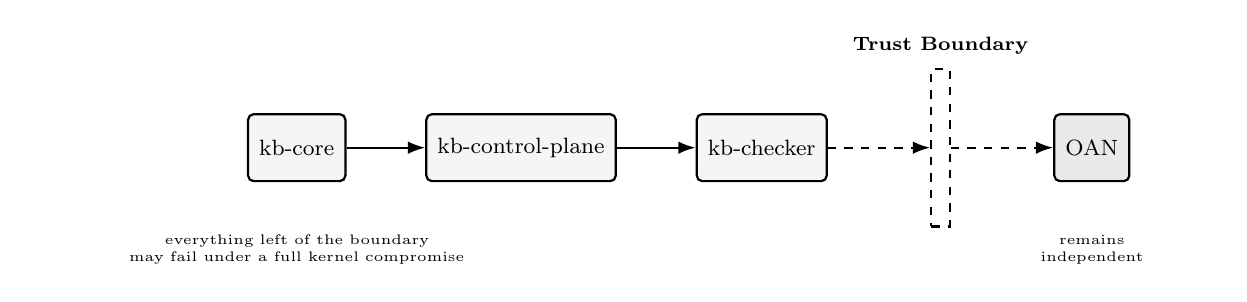
\begin{tikzpicture}[font=\footnotesize, node distance=1.0cm]
  \node[hostblock] (core) {kb-core};
  \node[hostblock, right=of core] (cp) {kb-control-plane};
  \node[hostblock, right=of cp] (kbc) {kb-checker};
  \draw[arr] (core) -- (cp);
  \draw[arr] (cp) -- (kbc);

  \node[draw=black, thick, dashed, minimum height=2.0cm, right=1.3cm of kbc] (boundary) {};
  \node[above=0.05cm of boundary, font=\scriptsize\bfseries] {Trust Boundary};

  \node[oanblock, right=1.3cm of boundary] (oan) {OAN};
  \draw[darr] (kbc) -- (boundary.west);
  \draw[darr] (boundary.east) -- (oan);

  \node[below=0.55cm of core, font=\tiny, align=center, text width=6.6cm] {everything left of the boundary\\may fail under a full kernel compromise};
  \node[below=0.55cm of oan, font=\tiny, align=center, text width=3.0cm] {remains\\independent};
\end{tikzpicture}
\figcap{Everything to the left of the trust boundary shares one kernel, and so shares one failure mode. OAN is the only component structurally guaranteed to still be telling the truth on the right.}
\label{fig:boundary}
\end{figure}

% =====================================================================
\section{The Recovery Ladder}
\label{sec:recovery}

Hardware fencing is the \emph{last} resort, not the first. It sits at
the bottom of a five-stage recovery ladder, built on top of
\texttt{kb-checker}'s existing three-stage software chain
(\texttt{systemctl stop} $\to$ \texttt{SIGKILL} $\to$ \texttt{iptables}
drop). OAN owns only the final stage.

\begin{figure}[h!]
\centering
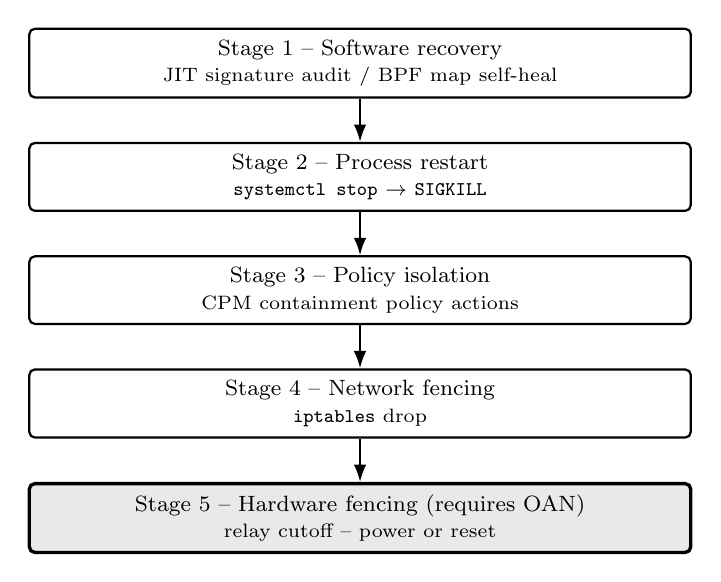
\begin{tikzpicture}[font=\footnotesize, node distance=0.55cm]
  \node[block, minimum width=8.4cm] (s1) {Stage 1 -- Software recovery\\\scriptsize JIT signature audit / BPF map self-heal};
  \node[block, below=of s1, minimum width=8.4cm] (s2) {Stage 2 -- Process restart\\\scriptsize \texttt{systemctl stop} \(\to\) \texttt{SIGKILL}};
  \node[block, below=of s2, minimum width=8.4cm] (s3) {Stage 3 -- Policy isolation\\\scriptsize CPM containment policy actions};
  \node[block, below=of s3, minimum width=8.4cm] (s4) {Stage 4 -- Network fencing\\\scriptsize \texttt{iptables} drop};
  \node[oanblock, below=of s4, minimum width=8.4cm, very thick] (s5) {Stage 5 -- Hardware fencing (requires OAN)\\\scriptsize relay cutoff -- power or reset};

  \draw[arr] (s1) -- (s2);
  \draw[arr] (s2) -- (s3);
  \draw[arr] (s3) -- (s4);
  \draw[arr] (s4) -- (s5);
\end{tikzpicture}
\figcap{The recovery ladder. Stages 1--4 are entirely within \texttt{kb-checker}'s existing software authority; only Stage 5 needs OAN, and only after every stage above it has already failed.}
\label{fig:ladder}
\end{figure}

Because Stage 5 sits strictly below the existing chain, a healthy host
never reaches OAN's relay at all --- the four software stages above it
already resolve the overwhelming majority of incidents on their own.

% =====================================================================
\section{Scaling to a Fleet: the Shared Chassis Design}
\label{sec:scaling}

A single OAN unit protects a single host. Most real deployments protect
more than one machine, so OAN's reference architecture is a
\textbf{shared chassis}: one physical box that supervises up to
\textbf{five hosts} at once, capped deliberately rather than grown
further.

\begin{figure}[h!]
\centering
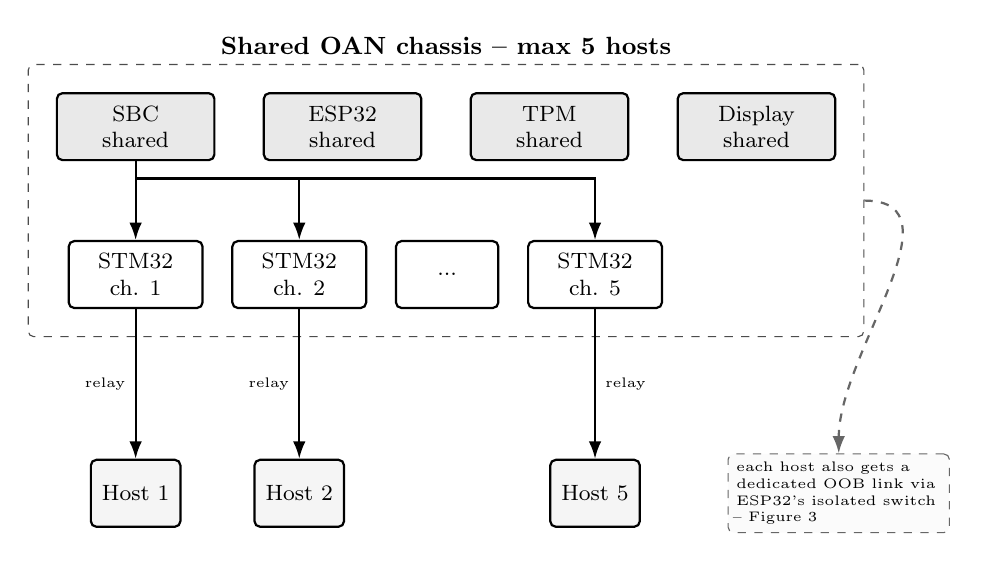
\begin{tikzpicture}[font=\scriptsize, node distance=0.5cm and 0.6cm]

  \node[oanblock, minimum width=2.0cm] (sbc) {SBC\\shared};
  \node[oanblock, right=of sbc, minimum width=2.0cm] (esp) {ESP32\\shared};
  \node[oanblock, right=of esp, minimum width=2.0cm] (tpm) {TPM\\shared};
  \node[oanblock, right=of tpm, minimum width=2.0cm] (disp) {Display\\shared};

  \node[block, below=1.0cm of sbc, minimum width=1.7cm] (c1) {STM32\\ch. 1};
  \node[block, right=0.35cm of c1, minimum width=1.7cm] (c2) {STM32\\ch. 2};
  \node[block, right=0.35cm of c2, minimum width=1.3cm] (c3) {...};
  \node[block, right=0.35cm of c3, minimum width=1.7cm] (c5) {STM32\\ch. 5};

  \draw[arr] (sbc.south) -- ++(0,-0.22) -| (c1.north);
  \draw[arr] (sbc.south) -- ++(0,-0.22) -| (c2.north);
  \draw[arr] (sbc.south) -- ++(0,-0.22) -| (c5.north);

  \node[groupbox, fit=(sbc)(esp)(tpm)(disp)(c1)(c2)(c3)(c5), inner sep=0.35cm, label={[font=\small\bfseries]above:Shared OAN chassis -- max 5 hosts}] (chassis) {};

  \node[hostblock, below=1.9cm of c1] (h1) {Host 1};
  \node[hostblock, below=1.9cm of c2] (h2) {Host 2};
  \node[hostblock, below=1.9cm of c5] (h5) {Host 5};

  \draw[arr] (c1.south) -- node[left, font=\tiny]{relay} (h1.north);
  \draw[arr] (c2.south) -- node[left, font=\tiny]{relay} (h2.north);
  \draw[arr] (c5.south) -- node[right, font=\tiny]{relay} (h5.north);

  \node[draw=black!60, dashed, rounded corners=2pt, fill=gray!3, right=1.1cm of h5,
    font=\tiny, align=left, text width=2.6cm, inner sep=3pt] (oobnote)
    {each host also gets a dedicated OOB link via ESP32's isolated switch -- Figure~3};
  \draw[darr, black!60] (chassis.east) to[out=0, in=90] (oobnote.north);
\end{tikzpicture}
\figcap{One shared chassis, up to five hosts. Each STM32 channel's relay wire is the fencing path; the OOB attestation link to each host runs separately through ESP32's isolated switch, detailed in Figure~3.}
\label{fig:chassis}
\end{figure}

\subsection{What Is Shared, and What Every Host Still Needs}

Sharing the chassis removes \emph{redundant} hardware, not per-host
hardware --- fencing and attestation are inherently host-specific, so
every host still needs its own physical wiring.

\begin{center}
\renewcommand{\arraystretch}{1.35}
\begin{tabular}{@{}p{5.4cm}p{8.2cm}@{}}
\toprule
\textbf{Shared once, across up to 5 hosts} & \textbf{Always required, per host} \\
\midrule
SBC (attestation engine, policy, dashboard) & A relay tap wired into that host's own power/reset header \\
ESP32 (owns the isolated switch port) & A dedicated OOB link endpoint --- a small dongle/NIC distinct from the host's normal network card \\
TPM (root of trust) & The STM32 channel logic watching that one link/relay pair \\
Display & Wiring and connectors specific to that host \\
\bottomrule
\end{tabular}
\end{center}

The transport for each host's channel is a dedicated, physically
isolated Ethernet segment --- its own small unmanaged switch, no uplink
to the production LAN --- rather than loose serial cables. This is
exactly the pattern enterprise BMC and IPMI~\cite{dmtfipmi} management networks already
use at this scale, for the same reason: physically and logically
separate from anything the host's own kernel drives. A VLAN carved out
of the host's \emph{own} NIC does not count as out-of-band, because the
host's kernel still drives that interface and can forge or block
traffic on it; each host's OOB link terminates on hardware distinct
from its main NIC.

\subsection{Why Cap at Five Hosts}

\begin{itemize}
  \item \textbf{Blast radius.} If the shared chassis itself fails or is
    physically tampered with, only five hosts lose OOB coverage at
    once, not an entire lab.
  \item \textbf{Commodity part sizes.} 5--8 channel relay/PDU boards
    and 5--8 port unmanaged switches are natural off-the-shelf sizes.
    Going bigger means custom boards instead of commodity ones.
  \item \textbf{USB/GPIO fan-out on the SBC.} A single-board computer's
    USB and GPIO budget gets cramped well before ten-plus channels; five
    keeps the shared SBC within what a stock board can drive without a
    custom PCB.
\end{itemize}

A lab of thirty machines is served by \textbf{six} shared chassis, each
independently reporting up to the fleet layer (\S\ref{sec:fms}) --- not
one giant chassis, and not thirty individual units.

% =====================================================================
\section{Fabric Management: One Node to a Fleet}
\label{sec:fms}

The Fabric Management Service (FMS) is the software layer, running on
the SBC (\S\ref{sec:sbc}), that turns many independent chassis into one
coordinated \textbf{Fabric}. It organizes protected systems into a
clean hierarchy.

\begin{figure}[h!]
\centering
\begin{forest}
for tree={
  draw=black, thick, rounded corners=2pt, fill=gray!8, font=\scriptsize,
  align=center, inner sep=3pt, l sep=11mm, s sep=5mm,
  edge={thick, -{Latex[length=1.6mm,width=1.2mm]}}
}
[Fabric
  [Colony A\\{\tiny one shared chassis}
    [Family A1\\{\tiny ``Linux Lab''}
      [Node] [Node] [Node]
    ]
    [Family A2\\{\tiny ``GPU''}
      [Node] [Node]
    ]
  ]
  [Colony B\\{\tiny another chassis}
    [Family B1
      [Node] [Node]
    ]
  ]
]
\end{forest}
\figcap{Fabric $\to$ Colony $\to$ Family $\to$ Node. A Colony maps directly onto one shared chassis (\S\ref{sec:scaling}); Families let administrators group hosts by purpose regardless of which chassis they are physically wired to.}
\label{fig:fabric}
\end{figure}

\begin{center}
\renewcommand{\arraystretch}{1.3}
\begin{tabular}{@{}p{2.6cm}p{11cm}@{}}
\toprule
\textbf{Term} & \textbf{Meaning} \\
\midrule
Fabric & The entire managed deployment --- every Colony, everywhere. \\
Colony & One shared chassis and the up-to-five hosts wired to it: a lab bench, a rack, a department. \\
Family & A logical grouping of Nodes by purpose (``AI Family'', ``Database Family''), independent of physical wiring. \\
Node & One protected host, running the full KB stack. \\
\bottomrule
\end{tabular}
\end{center}

\subsection{The Local Autonomy Principle}
\label{sec:autonomy}

\begin{notebox}[Local Autonomy Principle]
Every KB node remains fully capable of protecting itself without FMS.
\end{notebox}

FMS is never part of the runtime security path. Without it, every node
still has \texttt{kb-core}, \texttt{kb-control-plane}, \texttt{kb-checker},
local OAN attestation, local recovery, and local fencing --- nothing
about single-host protection changes. With FMS, the fleet additionally
gains visibility, policy synchronization, fleet-wide recovery
coordination, and a single inventory. Losing FMS costs coordination,
never protection:

\begin{center}
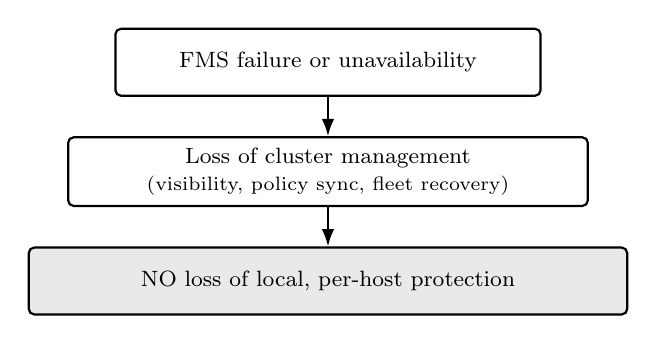
\begin{tikzpicture}[font=\footnotesize, node distance=0.5cm]
  \node[block, minimum width=5.4cm] (f) {FMS failure or unavailability};
  \node[block, below=of f, minimum width=6.6cm] (c) {Loss of cluster management\\\scriptsize (visibility, policy sync, fleet recovery)};
  \node[oanblock, below=of c, minimum width=7.6cm] (n) {NO loss of local, per-host protection};
  \draw[arr] (f) -- (c);
  \draw[arr] (c) -- (n);
\end{tikzpicture}
\end{center}

This is why FMS is classified \emph{operationally important, not
security-critical}, and why it runs entirely on the Fabric Management
Plane (\S\ref{sec:planes}), never on the OOB Trust Plane. An FMS outage
is an inconvenience; it is never a hole in a host's defenses.

\subsection{What Crosses the Fabric Plane}

FMS never receives raw kernel state. Each node reports a
\textbf{TPM-signed summary}, produced by the same trust chain described
in \S\ref{sec:tpm-relay} --- health, alerts, inventory, version, and
integrity status, and nothing more:

\begin{center}
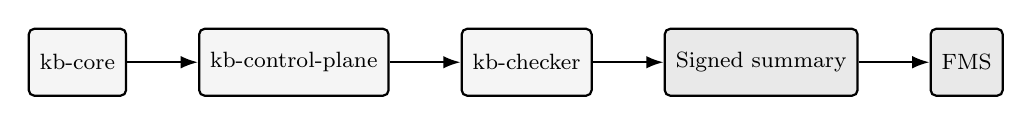
\begin{tikzpicture}[font=\footnotesize, node distance=0.9cm]
  \node[hostblock] (core) {kb-core};
  \node[hostblock, right=of core] (cp) {kb-control-plane};
  \node[hostblock, right=of cp] (kbc) {kb-checker};
  \node[oanblock, right=of kbc] (sum) {Signed summary};
  \node[oanblock, right=of sum] (fms) {FMS};
  \draw[arr] (core) -- (cp);
  \draw[arr] (cp) -- (kbc);
  \draw[arr] (kbc) -- (sum);
  \draw[arr] (sum) -- (fms);
\end{tikzpicture}
\end{center}

Because that summary is signed against the same TPM that already seals
both OAN's own state and the host's attestation (\S\ref{sec:tpm-relay}),
FMS can trust what it receives without ever needing raw access to
anything privileged --- and a compromised Fabric Management Plane still
cannot forge a clean report for a host that is actually compromised.

\subsection{Fleet Responsibilities}

\begin{center}
\renewcommand{\arraystretch}{1.3}
\begin{tabular}{@{}p{4.0cm}p{9.6cm}@{}}
\toprule
\textbf{Capability} & \textbf{What it does} \\
\midrule
Fabric Discovery & Finds new KB deployments automatically: registration, hardware fingerprinting, platform and version detection. \\
Node Registry & Keeps the inventory --- node ID, hostname, platform, kernel version, family, colony, health, trust status, last heartbeat. \\
Membership Management & Join/leave Fabric, node removal, family migration, colony reassignment. \\
Health Monitoring & Host availability, resource usage, \texttt{kb-core}/\texttt{kb-checker}/OAN connectivity, heartbeat. \\
Policy Management & Define a security policy once; deploy it to a Fabric, a Colony, a Family, or a single Node. \\
Event Aggregation & Unified timeline across every node --- search, indexing, historical record. \\
Cross-Host Correlation & Surfaces shared indicators and simultaneous anomalies across the fleet, in cooperation with \texttt{kb-aads}. \\
Recovery Coordination & Multi-node quarantine, fabric-wide recovery, controlled restart ordering. \\
Deployment Management & Version inventory, compatibility checks, controlled rollout. \\
\bottomrule
\end{tabular}
\end{center}

\subsection{Policy Inheritance}

Policy flows downward through the hierarchy, and a more specific level
can always override a broader default:

\begin{center}
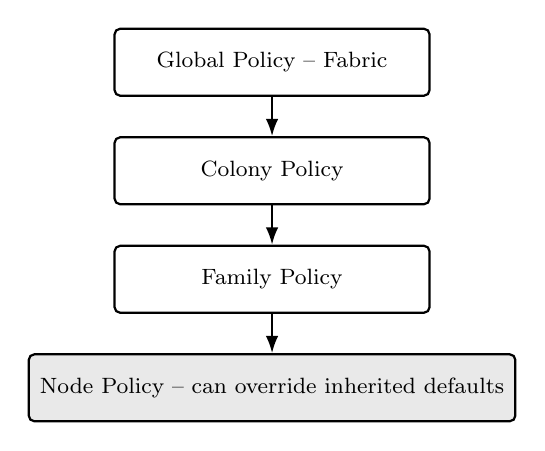
\begin{tikzpicture}[font=\footnotesize, node distance=0.5cm]
  \node[block, minimum width=4.0cm] (g) {Global Policy -- Fabric};
  \node[block, below=of g, minimum width=4.0cm] (c) {Colony Policy};
  \node[block, below=of c, minimum width=4.0cm] (f) {Family Policy};
  \node[oanblock, below=of f, minimum width=4.6cm] (n) {Node Policy -- can override inherited defaults};
  \draw[arr] (g) -- (c);
  \draw[arr] (c) -- (f);
  \draw[arr] (f) -- (n);
\end{tikzpicture}
\end{center}

Multiple Colonies never share a single point of failure at the trust
layer: each Colony keeps its own OAN chassis and its own FMS instance,
with no global master coordinating between them. A Colony stays
autonomous even if OANs are later given a way to synchronize with each
other for visibility --- autonomy is a property of the trust layer, not
a limitation on convenience features built above it.

% =====================================================================
\section{Deployment Walkthrough: From One Desk to a Lab}
\label{sec:walkthrough}

The shared-chassis design (\S\ref{sec:scaling}) is built so that a
single chassis grows smoothly from protecting one machine to protecting
five, without ever touching the shared hardware again once it is set
up. This section walks through that growth path in the order a team
would actually experience it.

\begin{center}
\renewcommand{\arraystretch}{1.4}
\small
\begin{tabular}{@{}p{1.1cm}p{5.0cm}p{7.3cm}@{}}
\toprule
\textbf{Stage} & \textbf{What happens} & \textbf{What already exists, reused as-is} \\
\midrule
1 & Assemble one shared chassis: SBC, ESP32, TPM, display, and the
dedicated OOB switch. & Nothing yet --- this is the one-time setup. \\
2 & Wire host \#1: relay tap into its power/reset header, dedicated
OOB dongle, one STM32 channel. Run the attestation heartbeat
(\S\ref{sec:heartbeat}) end to end. & The entire shared chassis from
Stage 1. \\
3 & Add hosts \#2 and \#3: repeat only the per-host wiring --- another
relay tap, another dongle, another STM32 channel. & SBC, ESP32, TPM,
display, switch --- unchanged. \\
4 & Fill the chassis: add hosts \#4 and \#5 the same way. The chassis
is now at its Pentagon cap (\S\ref{sec:scaling}). & Same shared
hardware, still unchanged since Stage 1. \\
5 & Organize with FMS: group the five Nodes into Families by purpose,
set Colony-level policy, and start collecting the signed-summary
event stream (\S\ref{sec:fms}). & All hardware from Stages 1--4; this
step is pure configuration. \\
6 & Scale past five: stand up a second, independent chassis for hosts
\#6--\#10, reporting to the same Fabric. & A second copy of Stage 1's
shared hardware --- deliberately \emph{not} an extension of the
first chassis (\S\ref{sec:scaling}'s cap rationale). \\
\bottomrule
\end{tabular}
\end{center}

\begin{plainbox}
Notice what never appears in the ``what happens'' column after Stage 1:
buying another SBC, another TPM, or another display. Every stage from 2
through 5 is wiring and configuration on top of hardware that was
bought exactly once. That is the whole economic argument for the
shared-chassis design, told as a sequence of actions instead of a cost
table (\S\ref{sec:bom} has the numbers).
\end{plainbox}

% =====================================================================
\section{Building One: Bill of Materials}
\label{sec:bom}

The numbers below describe a single shared chassis (\S\ref{sec:scaling})
built from commodity, off-the-shelf parts --- no custom silicon, no
board fabrication required to get a working unit on a bench. All INR
figures use an approximate \textasciitilde INR 87/USD conversion for
scoping; real domestic sourcing typically comes in lower.

\subsection{Shared Chassis Parts (bought once per chassis)}

\begin{center}
\renewcommand{\arraystretch}{1.3}
\small
\begin{tabular}{@{}p{4.6cm}p{5.2cm}rr@{}}
\toprule
\textbf{Component} & \textbf{Purpose} & \textbf{USD} & \textbf{INR} \\
\midrule
SBC (Raspberry Pi 4/5 or Intel N100) & Attestation engine, policy, dashboard, FMS & \$35--80 & INR 3,050--6,950 \\
microSD card (32GB+) & OS + watchdog binary & \$8 & INR 700 \\
ESP32 dev board & Management/comms processor & \$6--10 & INR 525--875 \\
Discrete TPM 2.0 module & Hardware root of trust & \$20--40 & INR 1,750--3,500 \\
I2C OLED/LCD display & Live status readout & \$5--10 & INR 440--875 \\
\midrule
\textbf{Shared total, per chassis} & & \textbf{\$74--148} & \textbf{INR 6,440--12,880} \\
\bottomrule
\end{tabular}
\end{center}

\subsection{Per-Host Channel Parts}

\begin{center}
\renewcommand{\arraystretch}{1.3}
\small
\begin{tabular}{@{}p{4.6cm}p{5.2cm}rr@{}}
\toprule
\textbf{Component} & \textbf{Purpose} & \textbf{USD} & \textbf{INR} \\
\midrule
STM32 dev board & That host's safety controller/relay channel & \$10--25 & INR 870--2,175 \\
Relay channel & Fencing for that host, on a shared multi-channel board & \$6 & INR 520 \\
OOB link hardware & Dedicated dongle/NIC, distinct from the host's main NIC & \$8 & INR 700 \\
Wiring/connectors & Cable run to that host & \$8 & INR 700 \\
\midrule
\textbf{Total, per host} & & \textbf{\$32--47} & \textbf{INR 2,785--4,090} \\
\bottomrule
\end{tabular}
\end{center}

\subsection{Total Cost by Fleet Size}

\begin{center}
\renewcommand{\arraystretch}{1.3}
\small
\begin{tabular}{@{}lccrr@{}}
\toprule
\textbf{Config} & \textbf{Hosts} & \textbf{Chassis} & \textbf{Total (USD)} & \textbf{Total (INR)} \\
\midrule
Single & 1 & 1 & \$106--195 & INR 9,220--16,965 \\
Triple & 3 & 1 & \$170--289 & INR 14,790--25,145 \\
Pentagon (cap) & 5 & 1 & \$234--383 & INR 20,360--33,320 \\
Lab & 30 & 6 & \$1,404--2,298 & INR 1,22,150--1,99,925 \\
\bottomrule
\end{tabular}
\end{center}

\begin{plainbox}
The shared parts (SBC, ESP32, TPM, display) are bought exactly once per
chassis, whether it is serving one host or all five. Every host past the
first only adds the \$32--47 per-host line --- which is why Pentagon's
per-\emph{host} cost (\$46.80--76.60) ends up under half of Single's
(\$106--195), even though Pentagon's per-\emph{person} cost is higher.
A team actually protecting more than one machine gets more coverage per
dollar by filling a chassis than by building single, standalone units.
\end{plainbox}

% =====================================================================
\section{Building It on a Budget}
\label{sec:budget}

The parts list above uses reasonable retail defaults, not the cheapest
possible build. A budget-constrained team can bring the shared-chassis
cost down substantially by swapping specific parts --- without touching
OAN's architecture or its guarantees.

\begin{center}
\renewcommand{\arraystretch}{1.3}
\small
\begin{tabular}{@{}p{3.9cm}rrr@{}}
\toprule
\textbf{Component} & \textbf{Reference} & \textbf{Budget} & \textbf{Swap} \\
\midrule
SBC & \$35--80 & \$15--20 & Pi Zero 2 W handles the workload comfortably \\
ESP32 & \$6--10 & \$3--5 & Bare WROOM module, no breakout board \\
STM32 & \$10--25 & \$3--6 & Bare ``Blue Pill'' clone \\
Relay & \$6/ch & \$4--6/ch & Shared multi-channel board \\
OOB dongle & \$8 & \$3--5 & Generic CP2102 clone \\
Display & \$5--10 & \$0 & Dropped entirely -- optional, non-decisional \\
\bottomrule
\end{tabular}
\end{center}

This brings a Pentagon (5-host) chassis down to roughly
\textbf{\$114--168 / INR 9,918--14,616} total --- about \$11.40--16.80 per
person for a team of ten.

\begin{figure}[h!]
\centering
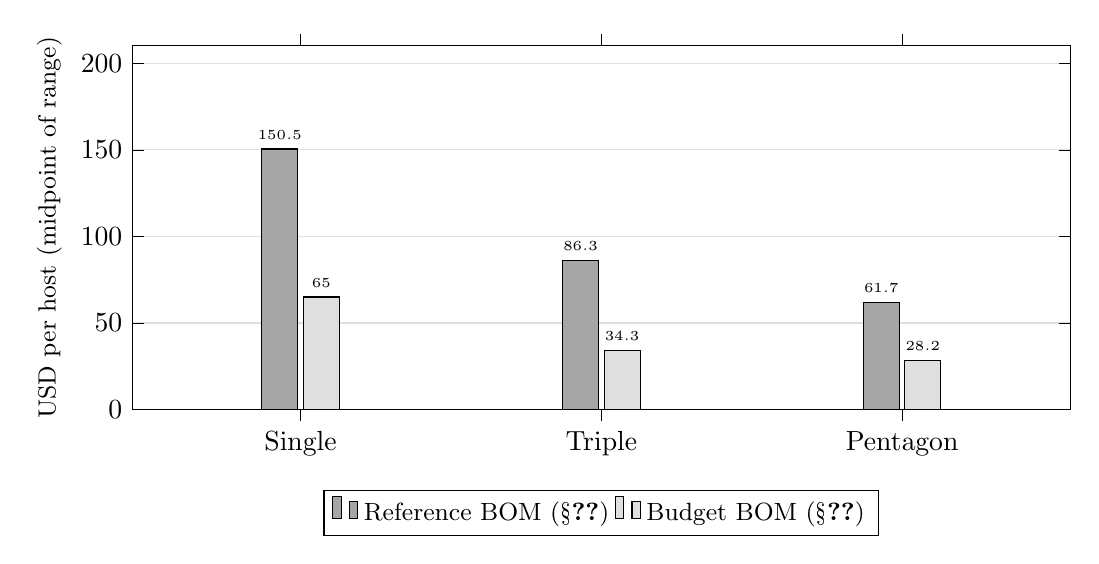
\begin{tikzpicture}
\begin{axis}[
  width=13.5cm, height=6.2cm,
  ybar, bar width=13pt,
  ymin=0, ymax=210,
  ylabel={USD per host (midpoint of range)},
  symbolic x coords={Single, Triple, Pentagon},
  xtick=data,
  legend style={at={(0.5,-0.22)}, anchor=north, legend columns=-1, font=\small},
  nodes near coords, every node near coord/.append style={font=\tiny},
  ymajorgrids, major grid style={gray!25},
  axis line style={black}, tick style={black}, every axis label/.style={font=\small},
  enlarge x limits=0.28
]
\addplot[fill=gray!70, draw=black] coordinates {(Single,150.5) (Triple,86.3) (Pentagon,61.7)};
\addplot[fill=gray!25, draw=black] coordinates {(Single,65.0) (Triple,34.3) (Pentagon,28.2)};
\legend{Reference BOM (\S\ref{sec:bom}), Budget BOM (\S\ref{sec:budget})}
\end{axis}
\end{tikzpicture}
\figcap{Per-host cost falls as a chassis fills, at both budget tiers, because the shared SBC/ESP32/TPM/display cost is the same regardless of how many of the five host slots are in use (\S\ref{sec:bom}'s ``Marginal Cost of Filling a Chassis'' logic).}
\label{fig:costchart}
\end{figure}

\begin{notebox}[What Stays, No Matter the Budget]
Two line items are never on the table, at any budget:

\begin{itemize}
  \item \textbf{The discrete TPM.} It is the one component whose entire
    job is being the thing a compromised host cannot fake. A software
    firmware-TPM would put OAN's own root of trust on the same silicon
    as its general-purpose SBC --- reintroducing, inside OAN itself,
    the exact same-failure-domain problem OAN exists to solve for the
    host.
  \item \textbf{The STM32 split.} Folding the watchdog and relay logic
    back onto the SBC to save a few dollars would recreate the ``the
    watchdog shares Linux's failure domain'' problem \S\ref{sec:stm32}
    exists specifically to avoid.
\end{itemize}
\end{notebox}

% =====================================================================
\section{The Production Appliance}
\label{sec:appliance-final}

Beyond the bench-buildable chassis, OAN's production form factor is a
single enclosed appliance:

\begin{figure}[h!]
\centering
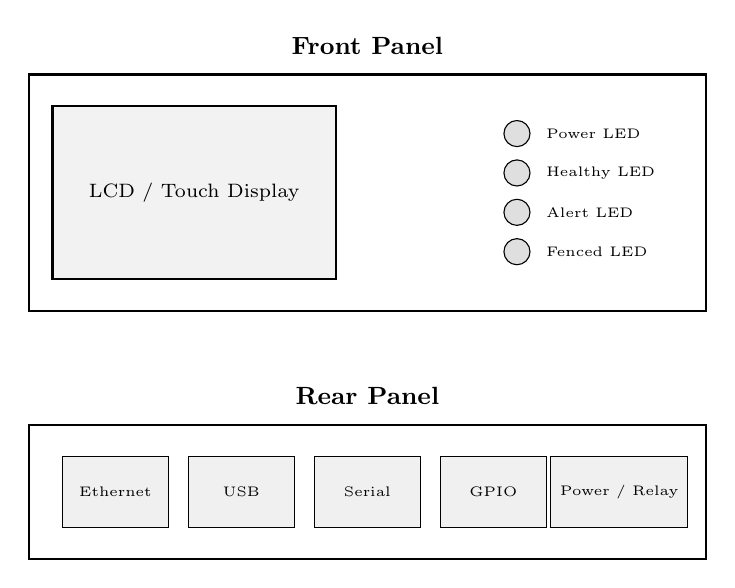
\begin{tikzpicture}[font=\scriptsize]
  \node[draw=black, thick, minimum width=8.6cm, minimum height=3.0cm] (front) at (0,1.9) {};
  \node[above=0.12cm of front, font=\small\bfseries] {Front Panel};

  \node[draw=black, thick, minimum width=3.6cm, minimum height=2.2cm, fill=gray!10] at ($(front)+(-2.2,0)$) (lcd) {LCD / Touch Display};
  \foreach \y/\txt in {0.75/Power, 0.25/Healthy, -0.25/Alert, -0.75/Fenced} {
    \node[draw=black, circle, minimum size=0.32cm, fill=gray!25] at ($(front)+(1.9,\y)$) {};
    \node[font=\tiny, anchor=west] at ($(front)+(2.15,\y)$) {\txt\ LED};
  }

  \node[draw=black, thick, minimum width=8.6cm, minimum height=1.7cm] at (0,-1.9) (rear) {};
  \node[above=0.12cm of rear, font=\small\bfseries] {Rear Panel};
  \foreach \x/\txt in {-3.2/Ethernet, -1.6/USB, 0/Serial, 1.6/GPIO, 3.2/{Power / Relay}} {
    \node[draw=black, minimum width=1.35cm, minimum height=0.9cm, fill=gray!12, font=\tiny, align=center] at ($(rear)+(\x,0)$) {\txt};
  }
\end{tikzpicture}
\figcap{Front panel gives a technician an at-a-glance read of host state; rear panel exposes every physical interface described in \S\ref{sec:architecture}--\S\ref{sec:tpm-relay}. Neither panel is on the trust-critical path -- both are read-outs and connectors, never decision inputs.}
\label{fig:appliance}
\end{figure}

\begin{center}
\renewcommand{\arraystretch}{1.3}
\begin{tabular}{@{}p{6.5cm}p{6.5cm}@{}}
\toprule
\textbf{Front panel} & \textbf{Rear panel} \\
\midrule
LCD / touch display & Ethernet \\
Power LED & USB \\
Healthy LED & Serial \\
Alert LED & GPIO \\
Fenced LED & Power, relay connector \\
\bottomrule
\end{tabular}
\end{center}

Internally, the SBC, STM32, ESP32, TPM, relay board, cooling, and power
regulation are all enclosed as one hardware unit -- the same
architecture as the bench chassis (\S\ref{sec:scaling}), packaged for a
rack or a desk rather than loose dev boards on a breadboard.

% =====================================================================
\section{Why This Architecture Works}

Every component in OAN has exactly one job, and no component both makes
the security decision and runs the general-purpose networked operating
system:

\begin{center}
\renewcommand{\arraystretch}{1.35}
\begin{tabular}{@{}lp{9.6cm}@{}}
\toprule
\textbf{Component} & \textbf{Responsibility} \\
\midrule
SBC & Decision-making, attestation, fleet management \\
STM32 & Deterministic safety, watchdog, relay control \\
ESP32 & Management communication and provisioning \\
TPM & Hardware trust anchor for both OAN and the host \\
Relay & Physical host fencing \\
Display & Local, read-only operational interface \\
\bottomrule
\end{tabular}
\end{center}

That separation is what lets OAN make a claim no purely-software
watchdog can: even if the SBC crashes, even if the ESP32 is fully
compromised over the network, and even if the host's own kernel is
lying about everything it reports, the STM32 still keeps its clock, the
TPM still keeps its keys, and the relay still works.

% =====================================================================
\section{Security Properties and Honest Limits}
\label{sec:properties}

A design is only as trustworthy as its stated boundaries. This section
makes both halves explicit: what OAN guarantees, and what it
deliberately leaves to other parts of Kernel Borderlands.

\subsection{What OAN Guarantees}

\begin{center}
\renewcommand{\arraystretch}{1.35}
\small
\begin{tabular}{@{}p{5.4cm}p{8.2cm}@{}}
\toprule
\textbf{Guarantee} & \textbf{Why it holds} \\
\midrule
Detection of a fully compromised host kernel & The heartbeat
(\S\ref{sec:heartbeat}) never routes through the host's kernel to
reach OAN -- there is no code path for a compromised kernel to
intercept. \\
Fencing that does not require host cooperation & The relay is wired to
the STM32, which never runs code the host can influence
(\S\ref{sec:stm32}). \\
Tamper-evidence of OAN's own state & Sealed against the TPM, covering
both OAN's own boot state and the host's reported measurements
(\S\ref{sec:tpm-relay}). \\
Fleet coordination that cannot weaken any single host & The Local
Autonomy Principle (\S\ref{sec:autonomy}) makes this true by
construction, not by discipline. \\
\bottomrule
\end{tabular}
\end{center}

\subsection{What OAN Does Not Do}

\begin{itemize}
  \item \textbf{It does not detect intrusions.} That is
    \texttt{kb-core}, \texttt{kb-control-plane}, and \texttt{kb-aads}'s
    job. OAN only verifies that the components doing that job are
    themselves still honest -- it has no opinion on process behavior,
    network traffic, or file activity.
  \item \textbf{It does not protect against physical access to itself.}
    A chassis that an attacker can physically open, rewire, or replace
    is a different threat model (physical security of the room),
    outside OAN's own scope.
  \item \textbf{It does not eliminate the need for the four software
    recovery stages.} OAN is Stage 5 of five (\S\ref{sec:recovery}) --
    the overwhelming majority of real incidents are expected to resolve
    at Stages 1--4, long before OAN's relay is ever involved.
  \item \textbf{It does not make the Fabric Management Plane
    trust-critical.} FMS coordinates; it never authorizes
    (\S\ref{sec:fms}).
\end{itemize}

\begin{plainbox}
A useful one-line summary: OAN answers exactly one question --
``can I still trust what this host is telling me?'' -- and answers it
in a way a fully compromised host cannot fake. It intentionally does
not try to answer any other question.
\end{plainbox}

% =====================================================================
\section{What-if: Boot/Rootkits?}
\label{sec:whatif}

Every guarantee in \S\ref{sec:properties} rests on one witness:
\texttt{kb-checker}. So the sharpest question this whole design
invites is the one this section answers: \emph{what if
\texttt{kb-checker} itself is lying?} Not killed, not silent --
compromised, and still talking.

\subsection{The Question, Stated Precisely}

\begin{analogybox}
A courtroom only works if the witness is telling the truth. A locked
door on the witness stand doesn't help if someone has already gotten
to the witness before they walked in. OAN's heartbeat
(\S\ref{sec:heartbeat}) is that witness stand -- and up to this point,
every guarantee this document has made assumes the witness is honest.
This section is about what happens the moment that assumption breaks.
\end{analogybox}

If an attacker achieves full kernel (Ring 0) compromise, they are not
outside \texttt{kb-checker}'s world -- they are underneath it. Every
fact \texttt{kb-checker} observes -- process lists, loaded modules,
BPF map contents, \texttt{/proc} entries -- ultimately comes from the
same kernel the attacker now controls. That opens two structurally
different failure modes, and the design so far has only answered one
of them well.

\begin{figure}[h!]
\centering
\resizebox{\linewidth}{!}{%
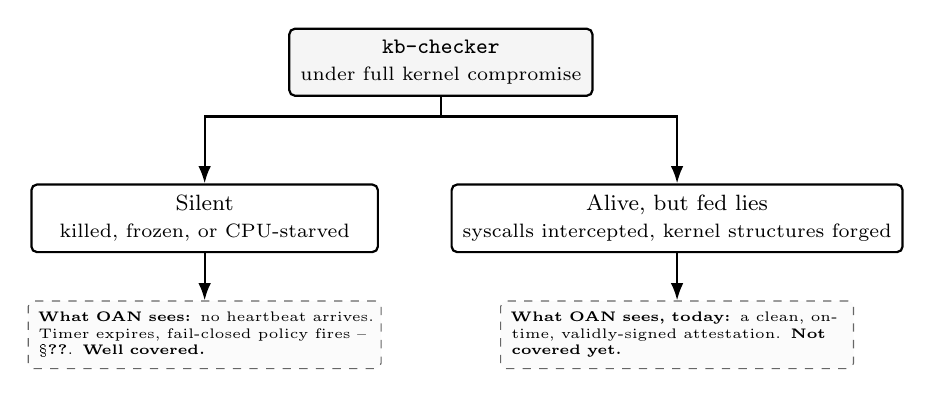
\begin{tikzpicture}[node distance=0.6cm and 1.3cm, font=\footnotesize]
  \node[hostblock, minimum width=3.6cm] (kbc) {\texttt{kb-checker}\\\scriptsize under full kernel compromise};

  \node[block, below=1.1cm of kbc, xshift=-3.0cm, minimum width=4.4cm] (silent) {Silent\\\scriptsize killed, frozen, or CPU-starved};
  \node[block, below=1.1cm of kbc, xshift=3.0cm, minimum width=4.4cm] (lying) {Alive, but fed lies\\\scriptsize syscalls intercepted, kernel structures forged};

  \draw[arr] (kbc.south) -- ++(0,-0.25) -| (silent.north);
  \draw[arr] (kbc.south) -- ++(0,-0.25) -| (lying.north);

  \node[draw=black!60, dashed, rounded corners=2pt, fill=gray!3, below=0.6cm of silent,
    font=\tiny, align=left, text width=4.2cm, inner sep=4pt] (silentnote)
    {\textbf{What OAN sees:} no heartbeat arrives. Timer expires, fail-closed policy fires -- \S\ref{sec:heartbeat}. \textbf{Well covered.}};
  \node[draw=black!60, dashed, rounded corners=2pt, fill=gray!3, below=0.6cm of lying,
    font=\tiny, align=left, text width=4.2cm, inner sep=4pt] (lyingnote)
    {\textbf{What OAN sees, today:} a clean, on-time, validly-signed attestation. \textbf{Not covered yet.}};

  \draw[arr] (silent.south) -- (silentnote.north);
  \draw[arr] (lying.south) -- (lyingnote.north);
\end{tikzpicture}%
}
\figcap{Two structurally different failures hiding behind one name. Silence is a solved problem -- the STM32's timer doesn't care why the heartbeat stopped, only that it did. A \texttt{kb-checker} that stays alive and keeps signing, fed false inputs by the kernel underneath it, is the harder case this section is about.}
\label{fig:twofailures}
\end{figure}

\textbf{Silence} is already solved, structurally, by \S\ref{sec:heartbeat}: the STM32's liveness timer never took input from the host to begin with, so it doesn't need to know \emph{why} the heartbeat stopped, only that it did.

\textbf{Lying} is harder, because a compromised kernel can feed
\texttt{kb-checker} forged answers to the exact syscalls it uses to
check on \texttt{kb-core} and itself, and \texttt{kb-checker} -- running its
real, unmodified code -- will faithfully sign and send an attestation
that is, from its own vantage point, completely honest. This is a
confused-deputy problem~\cite{hardy1988}: \texttt{kb-checker}'s
\emph{code integrity} can be real while its \emph{inputs} are poisoned
below the layer it can see.

\begin{notebox}[The Limit That Doesn't Move]
None of what follows makes \texttt{kb-checker} trustworthy again once
the kernel beneath it is compromised -- that is not achievable in
software, and this document will not pretend otherwise. What follows
narrows the set of attacks that can succeed \emph{without leaving a
detectable trace}, using components already in this design, at zero
additional hardware cost. The goal shifts from ``prevent the lie'' to
``make the lie expensive, and turn a failure into evidence.''
\end{notebox}

\subsection{Already Closed: Self-Containment}
\label{sec:cpm-closed}

One piece of this is already done, in the codebase, not just on paper.
The Critical Process Module's protected-component floor previously
covered \texttt{kb-sensor}, \texttt{kb-agent}, \texttt{kbctl},
\texttt{policy-engine}, and \texttt{dashboard} -- but not
\texttt{kb-checker}. That meant a malfunctioning or manipulated
detection engine could get \texttt{kb-checker} itself recommended for
containment through KB's \emph{own} pipeline, with nothing to stop it.
\texttt{kb-checker} (and \texttt{kbd}, which also covers CPM's
``policy-engine'' since policy evaluation runs inside the \texttt{kbd}
process) are now in CPM's compiled-in floor, with real, documented
install paths.

This closes a real gap, but it is worth being precise about which one:
CPM is an authorization gate in front of KB's \emph{own} containment
pipeline (\S2.4 of \texttt{CPM.md}, ``no self-containment, ever''). A
kernel-resident rootkit that never asks \texttt{contained\_pids\_map}
for permission -- because it corrupts scheduler state or task
structures directly -- never touches the path CPM guards. What it
\emph{does} buy: the ``silent'' bucket in
Figure~\ref{fig:twofailures} no longer has ``KB's own logic turned on
itself'' as a candidate cause. Silence now points more specifically at
something external.

\subsubsection{Hardening CPM's Own Data Structures}
\label{sec:bpf-map-hardening}

CPM's authorization gate is only as trustworthy as the BPF maps it
reads its decisions from. Both are now locked down at the map level,
not just guarded by convention:

\begin{itemize}
  \item \textbf{\texttt{BPF\_F\_RDONLY\_PROG} on
    \texttt{contained\_pids\_map} and
    \texttt{protected\_exec\_paths\_map}.} This flag restricts writes
    to the syscall boundary -- no in-kernel BPF program can write
    either map, only userspace can, over the existing
    \texttt{handle\_incoming\_containment\_cmd()} and
    \texttt{read\_cpm\_protected\_exec\_from\_bridge()} paths. A
    compromised or buggy BPF program -- a materially harder bar than
    a userspace exploit, given the verifier, but not an impossible one
    -- can read CPM's protected list but cannot forge an entry into
    it or clear \texttt{contained\_pids\_map} from the kernel side.
  \item \textbf{\texttt{bpf\_map\_freeze()} on
    \texttt{kb\_sensitive\_paths}.} Stronger than the flag above:
    freezing makes a map permanently read-only, from \emph{both}
    kernel and userspace, for the rest of that boot. Applied only to
    the one map that is genuinely done being written once startup
    finishes -- placed after the compiled-in floor populates it
    \emph{and} after the one-shot merge from \texttt{kbd} completes,
    immediately before the BPF programs attach.
\end{itemize}

\begin{notebox}[Why Not Freeze Everything]
\texttt{protected\_exec\_paths\_map} and
\texttt{protected\_workload\_paths\_map} stay unfrozen deliberately.
Both take legitimate writes \emph{after} startup -- an operator-pushed
overlay for the former, CWP's live workload-registration wire push for
the latter -- and freezing either would silently break a real feature
rather than close a gap. The distinction only holds if it's checked
against each map's actual write call sites individually; assuming
``looks similar, freeze it too'' is exactly the mistake this was built
to avoid. \texttt{bpf\_map\_freeze()} is also a best-effort step, not a
fatal one: if the freeze call itself fails, the sensor logs a warning
and continues unfrozen rather than refusing to start -- a hardening
step should not become a new availability risk on its own.
\end{notebox}

\subsection{Getting the Key Out of Host Memory}
\label{sec:key-in-tpm}

Before anything about detecting a lie: there is a sharper, more
immediate version of this problem worth closing first. If
\texttt{kb-checker}'s OOB signing key sits in its own process's RAM, a
Ring-0 attacker doesn't need \texttt{kb-checker} alive and lying at
all. They can read the key straight out of memory and forge
attestations directly -- or simply kill \texttt{kb-checker} and
impersonate it from then on, forever, with no watchdog left to notice.

\begin{notebox}[Which TPM]
Every mechanism in this and the next subsection uses the \emph{host's
own} TPM 2.0 -- physically on the protected machine, not OAN's. A TPM
can only make a hardware-backed statement about the machine it is
part of; OAN's own TPM (\S\ref{sec:tpm-relay}) can seal OAN's own
integrity and verify what \texttt{kb-checker} reports, but it cannot
attest to the host's measured-boot chain from across the OOB link --
there is no hardware path between them. Essentially every modern
server or workstation already ships with one, discrete or firmware
(Intel PTT~\cite{intelptt}, AMD fTPM~\cite{amdftpm}), for Secure Boot or disk encryption. Zero new
hardware, and no tension with \texttt{oan-cheap.md} \S3.7's rejection
of fTPM: that argument is specifically about not substituting the
host's fTPM for \emph{OAN's own} independent trust anchor. Using the
host's already-present TPM for a host-local job is a different
question, and this is precisely the case where a firmware TPM is
exactly what \texttt{oan-cheap.md} itself calls ``genuinely free.''
\end{notebox}

\begin{figure}[h!]
\centering
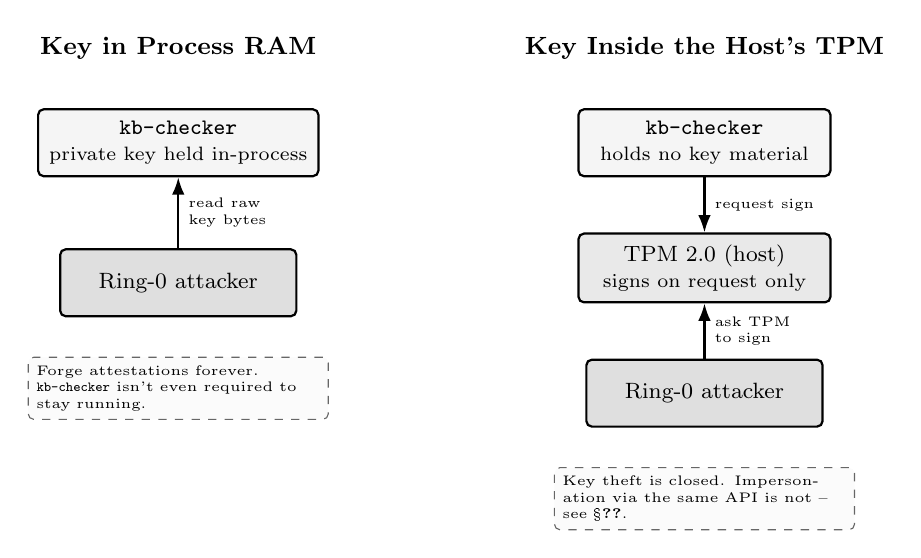
\begin{tikzpicture}[node distance=0.5cm and 0.6cm, font=\footnotesize]
  \node[font=\bfseries\small] (t1) {Key in Process RAM};
  \node[hostblock, below=0.5cm of t1, minimum width=3.4cm] (kbc1) {\texttt{kb-checker}\\\scriptsize private key held in-process};
  \node[block, below=0.9cm of kbc1, fill=gray!25, minimum width=3.0cm] (att1) {Ring-0 attacker};
  \draw[arr] (att1.north) -- (kbc1.south) node[midway, right, font=\tiny, align=left]{read raw\\key bytes};
  \node[draw=black!60, dashed, rounded corners=2pt, fill=gray!3, below=0.5cm of att1,
    font=\tiny, align=left, text width=3.6cm, inner sep=3pt]
    {Forge attestations forever. \texttt{kb-checker} isn't even required to stay running.};

  \node[font=\bfseries\small, right=2.4cm of t1] (t2) {Key Inside the Host's TPM};
  \node[hostblock, below=0.5cm of t2, minimum width=3.2cm] (kbc2) {\texttt{kb-checker}\\\scriptsize holds no key material};
  \node[oanblock, below=0.7cm of kbc2, minimum width=3.2cm] (tpm2) {TPM 2.0 (host)\\\scriptsize signs on request only};
  \node[block, below=0.7cm of tpm2, fill=gray!25, minimum width=3.0cm] (att2) {Ring-0 attacker};
  \draw[arr] (kbc2.south) -- (tpm2.north) node[midway, right, font=\tiny]{request sign};
  \draw[arr] (att2.north) -- (tpm2.south) node[midway, right, font=\tiny, align=left]{ask TPM\\to sign};
  \node[draw=black!60, dashed, rounded corners=2pt, fill=gray!3, below=0.5cm of att2,
    font=\tiny, align=left, text width=3.6cm, inner sep=3pt]
    {Key theft is closed. Impersonation via the same API is not -- see \S\ref{sec:pcr-seal}.};
\end{tikzpicture}
\figcap{The host's own TPM 2.0 -- already present on essentially any
modern server or workstation -- closes passive key theft for free:
have \texttt{kb-checker} request signing \emph{operations} rather than
holding raw key material. Zero new hardware; a protocol decision.}
\label{fig:keycustody}
\end{figure}

This is a protocol decision, not a bill-of-materials change -- the
host's own TPM is already there on essentially any real deployment
target. \texttt{kb-checker} asks it to sign; the private key never
exists in host RAM at all. But look closely at the right-hand side of
Figure~\ref{fig:keycustody}: a root-level attacker can still simply
place the \emph{same request} \texttt{kb-checker} would have made. The
TPM, by itself, doesn't know or care who is asking -- it only knows
what key was asked for. Key-in-TPM stops \emph{theft}. It does not, on
its own, stop \emph{impersonation}. That requires one more piece.

\FloatBarrier

\subsection{The Critical Piece: Sealing Key Usage to Measured Boot State}
\label{sec:pcr-seal}

This is the one mitigation in this section that doesn't just raise the
cost of a same-privilege-level attack -- it removes the attacker's
ability to use the key at all, for an entire class of compromise,
without \texttt{kb-checker} needing to notice anything.

\subsubsection{The Mechanism}

TPM 2.0 Platform Configuration Registers (PCRs)~\cite{tcgtpm2,tcgpcclient}
are not writable -- only \emph{extendable}: each measurement folds into
the register as $\mathrm{PCR}_{\text{new}} = H(\mathrm{PCR}_{\text{old}}
\Vert \text{measurement})$. This makes every PCR a one-way, cumulative
hash chain rooted at boot. Firmware measures itself, then measures the
bootloader; the bootloader measures the kernel image and initrd before
executing them; and, at runtime, the Integrity Measurement
Architecture (IMA)~\cite{sailer2004,kernelima} -- standard Linux, no
new hardware -- extends a PCR every time a kernel module loads.

\begin{figure}[h!]
\centering
\resizebox{\linewidth}{!}{%
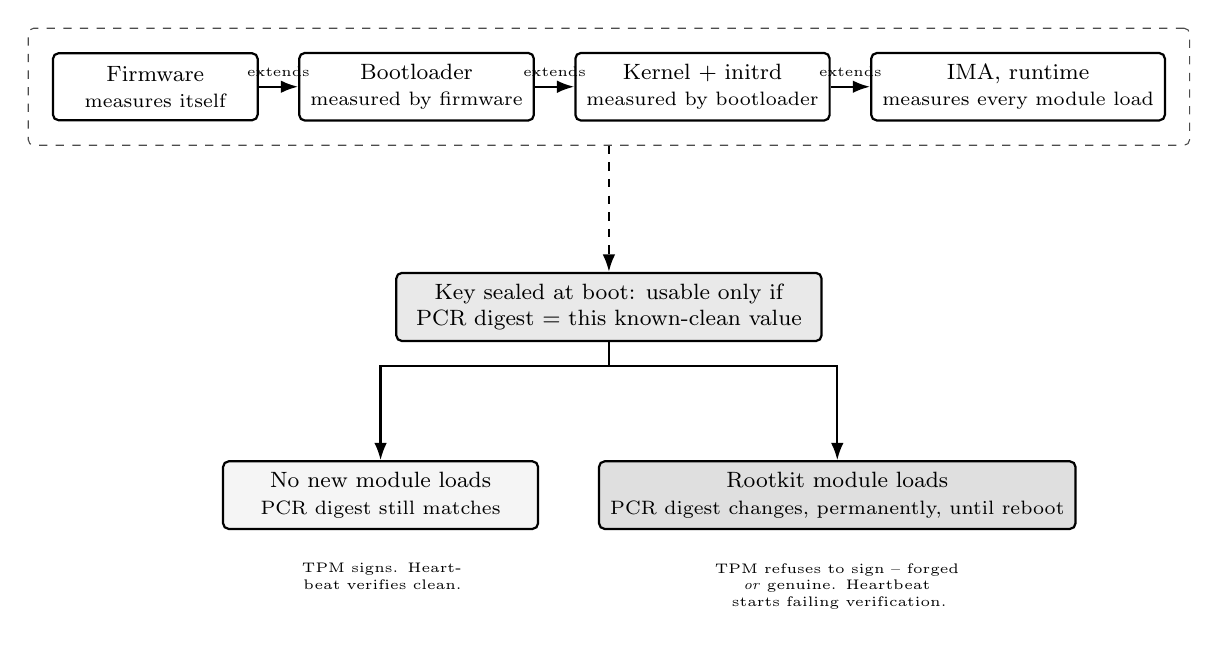
\begin{tikzpicture}[node distance=0.5cm and 0.5cm, font=\footnotesize]
  \node[block, minimum width=2.6cm] (fw) {Firmware\\\scriptsize measures itself};
  \node[block, right=of fw, minimum width=2.6cm] (bl) {Bootloader\\\scriptsize measured by firmware};
  \node[block, right=of bl, minimum width=2.8cm] (kern) {Kernel + initrd\\\scriptsize measured by bootloader};
  \node[block, right=of kern, minimum width=2.8cm] (ima) {IMA, runtime\\\scriptsize measures every module load};

  \draw[arr] (fw) -- node[above, font=\tiny]{extends} (bl);
  \draw[arr] (bl) -- node[above, font=\tiny]{extends} (kern);
  \draw[arr] (kern) -- node[above, font=\tiny]{extends} (ima);

  \node[groupbox, fit=(fw)(bl)(kern)(ima), inner sep=0.3cm] (chain) {};

  \node[oanblock, below=1.6cm of chain, minimum width=5.4cm] (sealed) {Key sealed at boot: usable only if\\PCR digest = this known-clean value};
  \draw[darr] (chain.south) -- (sealed.north);

  \node[hostblock, below=1.5cm of sealed, xshift=-2.9cm, minimum width=4.0cm] (clean) {No new module loads\\\scriptsize PCR digest still matches};
  \node[block, below=1.5cm of sealed, xshift=2.9cm, fill=gray!25, minimum width=4.0cm] (rootkit) {Rootkit module loads\\\scriptsize PCR digest changes, permanently, until reboot};

  \draw[arr] (sealed.south) -- ++(0,-0.3) -| (clean.north);
  \draw[arr] (sealed.south) -- ++(0,-0.3) -| (rootkit.north);

  \node[font=\tiny, align=center, below=0.3cm of clean, text width=3.8cm] {TPM signs. Heartbeat verifies clean.};
  \node[font=\tiny, align=center, below=0.3cm of rootkit, text width=4.0cm] {TPM refuses to sign -- forged \emph{or} genuine. Heartbeat starts failing verification.};
\end{tikzpicture}%
}
\figcap{The measured-boot chain, and what a rootkit module load does to it. PCRs only extend, never reset, short of a full platform reboot through the same chain -- so a rootkit cannot simply ``fix'' the value from inside the kernel it just compromised.}
\label{fig:pcrchain}
\end{figure}

A key can be created with a \texttt{TPM2\_PolicyPCR} authorization
policy: a digest computed over chosen PCR values at seal time. From
then on, the TPM performs a signing operation with that key only if
the \emph{current} PCR values, hashed the same way, match that digest
-- checked entirely inside the chip. There is no step in that sequence a
same-privilege-level attacker can intercept, because the attacker is
not inside the TPM.

\begin{figure}[h!]
\centering
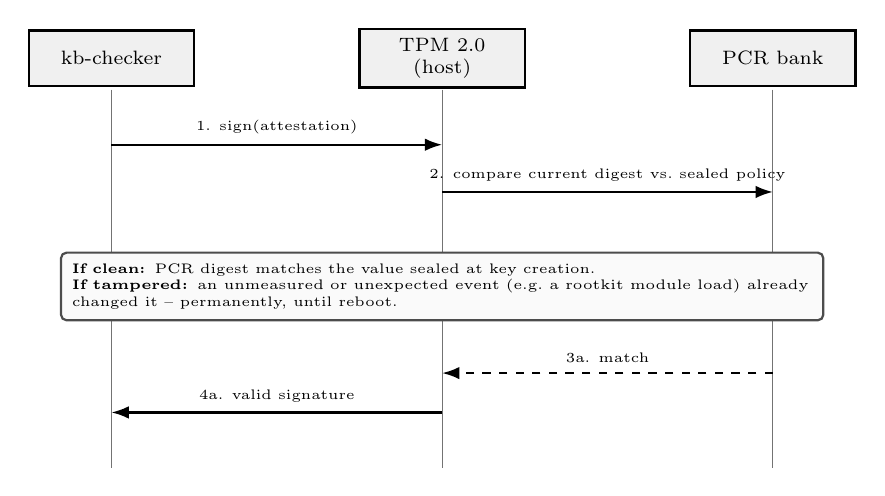
\begin{tikzpicture}[font=\scriptsize]
  \def\yTop{0}
  \def\yBot{-5.2}
  \node[actor] (kbc) at (0,\yTop) {kb-checker};
  \node[actor] (tpm) at (4.2,\yTop) {TPM 2.0\\\scriptsize (host)};
  \node[actor] (pcr) at (8.4,\yTop) {PCR bank};

  \foreach \x in {0,4.2,8.4}{
    \draw[lifeline] (\x,\yTop-0.4) -- (\x,\yBot);
  }

  \draw[arr] (0,-1.1) -- node[above, font=\tiny, align=center]{1. sign(attestation)} (4.2,-1.1);
  \draw[arr] (4.2,-1.7) -- node[above, font=\tiny]{2. compare current digest vs.\ sealed policy} (8.4,-1.7);

  \node[draw=black!70, thick, rounded corners=2pt, fill=gray!4, align=left,
    font=\tiny, text width=9.4cm, inner sep=4pt] at (4.2,-2.9)
    {\textbf{If clean:} PCR digest matches the value sealed at key creation.\\
     \textbf{If tampered:} an unmeasured or unexpected event (e.g.\ a rootkit module load) already changed it -- permanently, until reboot.};

  \draw[darr] (8.4,-4.0) -- node[above, font=\tiny, align=center]{3a. match} (4.2,-4.0);
  \draw[arr] (4.2,-4.5) -- node[above, font=\tiny]{4a. valid signature} (0,-4.5);
\end{tikzpicture}
\figcap{The PCR-sealed signing request. Step 2 happens inside the TPM chip itself -- the host never gets to answer ``is my boot state clean,'' it only gets told the result. On mismatch, the TPM returns an error instead of step 4a, for \emph{any} caller, forged or genuine.}
\label{fig:pcrsigning}
\end{figure}

\subsubsection{Before and After, From the Attacker's Side}

\begin{center}
\renewcommand{\arraystretch}{1.4}
\small
\begin{tabular}{@{}p{3.6cm}p{9.8cm}@{}}
\toprule
\textbf{Key custody} & \textbf{What the attacker needs} \\
\midrule
Key in process RAM & Any Ring-0 primitive, from any privilege-escalation
class. Read the key, forge forever. \\
Key in TPM, unsealed & Any Ring-0 primitive, plus the ability to call
the TPM's signing API -- trivial once root. Theft is closed;
impersonation is not. \\
Key in TPM, PCR-sealed & Ring-0 achieved via a path that never extends
the sealed PCRs -- narrowed from ``any privilege escalation'' down to
memory-corruption-only exploitation of \emph{already-loaded,
already-measured} code, with zero new modules, for as long as the
attacker wants to keep forging. \\
\bottomrule
\end{tabular}
\end{center}

\begin{plainbox}
The important property isn't just ``harder'' -- it's
\textbf{self-terminating}. A rootkit that needs to load anything, even
something auxiliary, even temporarily, doesn't get an error and a
chance to route around it while staying resident. The key goes dark
for the rest of that boot session, full stop, the moment the PCR
extends. Most real persistent Linux rootkits ship as loadable modules,
because writing durable kernel-level capability without ever loading
new code is a substantially harder engineering problem than the
alternative -- so this closes the well-trodden path, not a rare one.
\end{plainbox}

This is also what turns a bare fencing event into a specific claim
(\S\ref{sec:classify}): if the TPM starts refusing to sign, that is
not ``something is wrong, generically.'' It is ``the measured-boot
state changed since this key was sealed'' -- about as close to a
direct rootkit or bootkit signature as this design can produce without
new hardware.

\subsubsection{Demo Environment: Trying This on Real Hardware}
\label{sec:demo-env}

This mechanism is testable on unmodified, real hardware -- most
laptops and desktops built in the last several years already have
everything it needs.

\textbf{Checking for a TPM, on Linux:}

\begin{lstlisting}
ls /dev/tpm*                              # /dev/tpm0, /dev/tpmrm0 present?
cat /sys/class/tpm/tpm0/tpm_version_major # should print 2
dmesg | grep -i tpm                       # kernel's own boot-time detection
\end{lstlisting}

If nothing shows up, the chip may still exist but be disabled in
firmware (look for ``Intel PTT'' or ``AMD fTPM''/``Security Device'' in
BIOS/UEFI setup~\cite{uefispec}) -- a firmware setting, not a Linux one, so it needs a
reboot into setup, not a kernel config change. Install the tooling
needed for everything below:

\begin{lstlisting}
sudo pacman -S tpm2-tools     # Arch and derivatives
sudo apt install tpm2-tools   # Debian/Ubuntu
\end{lstlisting}
\noindent\texttt{tpm2-tools}, from the \texttt{tpm2-software}
project~\cite{tpm2software}, is the standard userspace CLI for TPM 2.0.

\begin{notebox}[Before Touching Anything]
Check first whether the machine already relies on the TPM for disk
encryption (\texttt{systemd-cryptenroll}, Clevis+Tang, or similar) --
creating or evicting TPM objects could interfere with an existing
unlock path. If none of that is in use, there is nothing to worry
about. Either way, the walkthrough below deliberately never touches
PCRs~0--10, the ones any real boot chain (firmware, bootloader,
kernel, IMA) actually measures into -- it uses PCR~16, one of a small
number the TCG spec~\cite{tcgpcr} defines as resettable ``debug'' registers,
untouched by any standard Linux boot and resettable without a reboot.
Confirm it is at its expected all-zero baseline first:
\end{notebox}

\begin{lstlisting}
tpm2_pcrread sha256:16
\end{lstlisting}

\textbf{The walkthrough.} Seal a secret to PCR~16's current value,
confirm it unseals cleanly, then extend that PCR the way a rootkit
module load would extend a real one, and watch the same unseal fail --
\S\ref{sec:pcr-seal}'s whole argument, live, without touching a real
kernel module or the boot chain the machine actually depends on:

\begin{lstlisting}
# 1. Primary key, owner hierarchy
tpm2_createprimary -C o -c primary.ctx

# 2. Trial session to compute the policy digest for "PCR 16 unchanged"
tpm2_startauthsession -S session.ctx
tpm2_policypcr -S session.ctx -l sha256:16 -L policy.digest
tpm2_flushcontext session.ctx

# 3. Seal a test secret under that policy
echo -n "test-secret" | tpm2_create -C primary.ctx -u seal.pub \
    -r seal.priv -L policy.digest -i-
tpm2_load -C primary.ctx -u seal.pub -r seal.priv -c seal.ctx

# 4. Real policy session, satisfy it, unseal -- should print "test-secret"
tpm2_startauthsession --policy-session -S session.ctx
tpm2_policypcr -S session.ctx -l sha256:16
tpm2_unseal -c seal.ctx -p session:session.ctx
tpm2_flushcontext session.ctx

# 5. Extend PCR 16 -- stand-in for an unmeasured/unexpected boot event
tpm2_pcrextend 16:sha256=$(echo -n "rootkit" | sha256sum | cut -d' ' -f1)

# 6. Same unseal, fresh session -- now fails
tpm2_startauthsession --policy-session -S session2.ctx
tpm2_policypcr -S session2.ctx -l sha256:16
tpm2_unseal -c seal.ctx -p session:session2.ctx
tpm2_flushcontext session2.ctx

# 7. Clean up -- PCR 16 resets without a reboot, unlike 0-15
tpm2_pcrreset 16
\end{lstlisting}

Step 6 is the demonstration: identical request, identical secret,
identical key -- the only thing that changed is the PCR value, and the
TPM refuses regardless of whether the request coming in is the
legitimate caller or an attacker replaying the exact same commands.
Exact flag names can shift slightly between \texttt{tpm2-tools}
releases; if a step errors, \texttt{man tpm2\_<command>} for the
installed version usually resolves it in one look.

\begin{notebox}[What This Does Not Close]
\begin{itemize}
  \item \textbf{Memory-corruption-only exploits.} An attack path that
    reaches Ring 0 purely through in-place patching of already-loaded,
    already-measured code -- no new module, ever -- extends no PCR and
    trips nothing. Narrower than ``any rootkit,'' not zero -- and
    narrower still once \S\ref{sec:memcorr-narrowing}'s mitigations are
    stacked on top.
  \item \textbf{Physical TPM bus sniffing.} A discrete TPM
    communicating over an unencrypted LPC/SPI bus is a documented
    attack class (the same category demonstrated against BitLocker on
    some hardware). It requires physical board access, not a remote
    exploit -- TPM 2.0 parameter-encryption sessions mitigate it, at
    zero new hardware cost, same as everything else in this section.
  \item \textbf{Upstream compromise of the measurement chain itself}
    (firmware, bootloader, Secure Boot bypass) is a different, higher-effort
    threat class this doesn't address -- and isn't really OAN's problem
    to solve; it's the layer OAN's own trust starts from.
  \item \textbf{Real operational cost.} Every legitimate kernel update
    or intentionally-added module requires re-sealing the key against a
    new expected PCR digest. That is a key-management process that has
    to actually exist and be exercised correctly -- skip it once and a
    routine patch locks the key out for no security reason; build a
    habit of re-sealing without checking \emph{why} the PCR changed,
    and the whole mechanism is quietly defeated.
\end{itemize}
\end{notebox}

\subsection{Narrowing the Memory-Corruption Gap}
\label{sec:memcorr-narrowing}

PCR-sealing leaves exactly one gap open: an attacker whose path to
Ring~0 never triggers a measured event. That isn't one attack, it's a
category -- and most of that category can be narrowed further with
mitigations that already ship in mainline Linux and mainstream
compilers, at zero new hardware cost. None of them close the gap
completely; nothing can. Each removes one specific technique from the
attacker's toolbox, and stacked together, what survives is a much
narrower thing than ``any memory-corruption bug.''

\begin{figure}[h!]
\centering
\resizebox{\linewidth}{!}{%
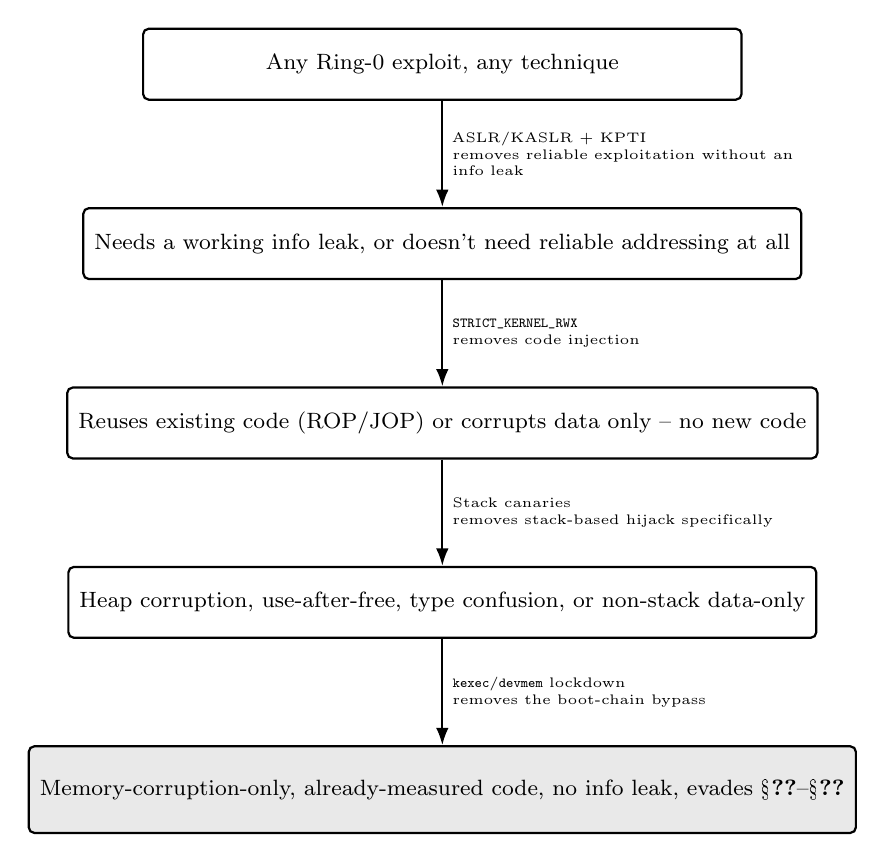
\begin{tikzpicture}[node distance=1.35cm, font=\footnotesize]
  \node[block, minimum width=7.6cm, minimum height=0.9cm] (b1) {Any Ring-0 exploit, any technique};
  \node[block, below=of b1, minimum width=7.6cm, minimum height=0.9cm] (b2) {Needs a working info leak, or doesn't need reliable addressing at all};
  \node[block, below=of b2, minimum width=7.6cm, minimum height=0.9cm] (b3) {Reuses existing code (ROP/JOP) or corrupts data only -- no new code};
  \node[block, below=of b3, minimum width=7.6cm, minimum height=0.9cm] (b4) {Heap corruption, use-after-free, type confusion, or non-stack data-only};
  \node[oanblock, below=of b4, minimum width=7.6cm, minimum height=1.1cm] (b5) {Memory-corruption-only, already-measured code, no info leak, evades \S\ref{sec:cross-consistency}--\S\ref{sec:clock-crosscheck}};

  \draw[arr] (b1) -- (b2) node[midway, right, font=\tiny, align=left, text width=4.4cm]{ASLR/KASLR + KPTI\\removes reliable exploitation without an info leak};
  \draw[arr] (b2) -- (b3) node[midway, right, font=\tiny, align=left, text width=4.4cm]{\texttt{STRICT\_KERNEL\_RWX}\\removes code injection};
  \draw[arr] (b3) -- (b4) node[midway, right, font=\tiny, align=left, text width=4.4cm]{Stack canaries\\removes stack-based hijack specifically};
  \draw[arr] (b4) -- (b5) node[midway, right, font=\tiny, align=left, text width=4.4cm]{\texttt{kexec}/\texttt{devmem} lockdown\\removes the boot-chain bypass};
\end{tikzpicture}%
}
\figcap{What's left after every free mitigation is stacked. Each layer removes one specific technique, not ``exploitation in general'' -- the box that survives at the bottom is deliberately still non-empty.}
\label{fig:narrowing}
\end{figure}

\subsubsection{Preventive Hardening, Already Mostly Free}

\textbf{ASLR/KASLR}~\cite{pax2003} randomizes where the kernel and its structures land
in memory on every boot. A memory-corruption bug that doesn't know
where anything is usually just crashes the machine rather than
achieving reliable code execution. \textbf{KPTI}'s role here is more
specific than it first looks: its actual job is closing Meltdown-class
speculative-execution reads of kernel memory from userspace~\cite{lipp2018} -- and one
of the most practical uses of that class of leak is defeating KASLR
before ever triggering the corruption bug~\cite{gruss2017}. KPTI's contribution to this
problem is indirect but real: it closes a common way an attacker turns
``crash'' into ``reliable exploit.''

\textbf{Stack canaries}~\cite{cowan1998} (\texttt{-fstack-protector} and family) place a
random value next to the return address on the stack; a stack buffer
overflow overwrites the canary before it reaches anything that
matters, and the check fails before the corrupted return address is
ever used. Scope-limited, precisely: this defends stack overflows
only, not heap corruption, use-after-free, or type confusion. A
stronger, hardware-backed version exists -- Intel CET's shadow stack
(\texttt{SHSTK})~\cite{intelcet} keeps a second, hardware-protected copy of return
addresses a regular overflow cannot touch -- but that specific
guarantee needs a CET-capable CPU. A software-only shadow stack exists
too, and is weaker; the two should not be conflated.

\textbf{\texttt{CONFIG\_STRICT\_KERNEL\_RWX}} enforces W\textasciicircum X
(write XOR execute)~\cite{deraadt2005} on kernel memory: once loaded, code pages are
read-only and executable, data pages are non-executable. This directly
blocks the classic ``corrupt memory, inject shellcode, jump to it''
technique~\cite{solardesigner1997}. It is precisely scoped, and precisely limited:
\textbf{return-oriented~\cite{shacham2007} and jump-oriented programming (ROP/JOP)~\cite{bletsch2011}, and
data-only attacks, inject no new code at all.} They redirect control
flow to reuse code that is already legitimately executable, or corrupt
data structures -- credentials, function pointers -- without touching
a code page. W\textasciicircum X is silent on both. This is the
sharpest technique that survives every mitigation on this list at
once, and it is what Figure~\ref{fig:narrowing}'s bottom box is built
from.

\begin{notebox}[Compatibility, Not Just Security]
\texttt{CONFIG\_STRICT\_KERNEL\_RWX} can break legacy or out-of-tree
kernel modules that expect to self-modify code at runtime. This is a
one-time compatibility check against your actual driver set at
deployment, not an ongoing operational risk -- unlike the trade-off in
\S\ref{sec:lkrg-report-only} below.
\end{notebox}

\subsubsection{Confirmed on kb-core's Own Userspace Daemon}
\label{sec:kbcore-hardening-confirmed}

The mitigations above are described in general terms; kb-core's
own userspace loader/bridge -- \texttt{kbd\_sensor} and its six
collector binaries, the code that manages CPM's BPF maps
(\S\ref{sec:bpf-map-hardening}) and loads the eBPF programs its LSM
hooks run as -- now actually carries them, confirmed against the
compiled output rather than assumed from the build flags:

\begin{itemize}
  \item \texttt{-fPIE}/\texttt{-pie}: the userspace equivalent of
    KASLR above, applied to all 7 of kb-core's build targets.
  \item \texttt{-fstack-protector-strong} and
    \texttt{-fstack-clash-protection}: stack canaries, plus protection
    against stack-clash allocation attacks -- the latter not covered
    anywhere above.
  \item \texttt{-D\_FORTIFY\_SOURCE=3}: compile- and runtime bounds
    checking on common libc calls (\texttt{memcpy}, \texttt{sprintf},
    and similar), including cases where the object size is only known
    at runtime -- the strongest variant, requiring \texttt{-O1} or
    higher to take effect.
  \item \texttt{-Wl,-z,relro,-z,now}: full RELRO. Resolves every
    dynamic symbol at load time and marks the GOT read-only
    immediately rather than lazily -- the userspace analog of
    \texttt{CONFIG\_STRICT\_KERNEL\_RWX}'s protection, applied to a
    different writable target (the GOT, not kernel code pages)
    against the same class of overwrite-and-redirect technique.
\end{itemize}

Confirmed against the actual binary, not just the Makefile:
\texttt{readelf -h} for \texttt{ET\_DYN} (PIE), \texttt{readelf -d}
for \texttt{BIND\_NOW}, and \texttt{nm} for
\texttt{\_\_stack\_chk\_fail}, after a full \texttt{make clean \&\&
make}. A flag that looks correct in a Makefile and doesn't survive a
sub-make, a flag-ordering issue, or a silently-ignored unsupported
flag is a real, recurring way hardening passes fail without anyone
noticing -- checking the compiled output is what closes that loop.

\subsubsection{Closing the Bypass in the Measured-Boot Chain Itself}

\S\ref{sec:pcr-seal}'s entire guarantee assumes new code only enters
the kernel through a path IMA measures. \texttt{kexec} is a
documented way around that assumption: \texttt{kexec\_load} boots a
completely different kernel image without a hardware reset, and
without ever going back through firmware or bootloader measurement --
the PCR values would simply never reflect it. The fix isn't
necessarily disabling \texttt{kexec} outright: Linux's
\texttt{kernel\_lockdown} LSM~\cite{kernellockdown} already gates \texttt{kexec\_load} and
permits \texttt{kexec\_file\_load} only for images signed by a trusted
key~\cite{kernelmodsig} -- the same signature-enforcement principle
\S\ref{sec:pcr-seal} already leans on for modules, applied to the one
other path that can introduce an unmeasured kernel. Restricting
\texttt{/dev/mem} and \texttt{/dev/kmem} (\texttt{CONFIG\_STRICT\_DEVMEM})
closes the more direct version of the same problem: unrestricted, either
lets a sufficiently privileged process read or write physical memory
directly, bypassing every mitigation in this section at once.

\subsubsection{What Survives All of It: a Same-Privilege-Level Last Resort}
\label{sec:lkrg-report-only}

Stacked, the mitigations above narrow the surviving attack down to a
ROP/JOP or data-only exploit against already-loaded, already-measured
code, with no accompanying info leak, evading the cross-checks in
\S\ref{sec:cross-consistency}--\S\ref{sec:clock-crosscheck}. That is a
substantially harder, more specific attacker than ``any memory
corruption,'' but it is not zero -- and for exactly that residual
sliver, an active kernel-resident integrity monitor such as Linux
Kernel Runtime Guard (LKRG)~\cite{lkrg} can still add value, with one important
condition on how it's deployed.

LKRG snapshots kernel \texttt{.text} and critical structures (process
credentials, security module state) and re-validates them on a mix of
timer ticks and hooked kernel events. It is a real, existing project,
and its own honest limitation is a race: LKRG runs at the \emph{same}
privilege level as the exploit it's trying to catch. An attacker fast
enough to disable or patch out LKRG before its next check wins. This
puts LKRG in a fundamentally different category from
\S\ref{sec:pcr-seal}'s PCR-sealing -- it is the one mechanism in this
whole document explicitly \emph{not} a same-privilege-level
countermeasure; LKRG explicitly is one.

\begin{notebox}[Report, Don't Enforce]
LKRG's more aggressive response modes -- killing the offending process,
or panicking the box on detection -- are a real, documented
availability risk for a production server, and a fair reason to rule
it out entirely if that's the only mode on offer. It isn't: run LKRG in
logging/alert-only mode, and treat its findings the same way this
document treats every other same-privilege-level signal -- as one more
contributor to the \emph{content implausibility} bucket in
\S\ref{sec:classify}, not as an autonomous enforcement action. The one
place that gets to take a disruptive action stays OAN's own
deliberately-chosen fail-open/fail-closed relay policy
(\S\ref{sec:tpm-relay}) -- not a second, uncoordinated kill switch
racing the attacker inside the kernel on its own terms. Deployed this
way, LKRG must also be part of the measured baseline itself, loaded
early enough that its own presence is expected at PCR-seal time, not
an unmeasured surprise.
\end{notebox}

\begin{center}
\renewcommand{\arraystretch}{1.5}
\small
\begin{tabular}{@{}p{3.2cm}p{5.7cm}p{4.1cm}@{}}
\toprule
\textbf{Layer} & \textbf{Removes} & \textbf{Cost / caveat} \\
\midrule
ASLR / KASLR + KPTI & Reliable exploitation without a separate info
leak & Near zero; on by default on most current kernels \\
\texttt{STRICT\_KERNEL\_RWX} & Code-injection exploitation & May break
legacy/out-of-tree modules; silent on ROP/JOP/data-only \\
Stack canaries & Stack-based control-flow hijack & Sub-1\% overhead;
scope-limited to stack overflows \\
\texttt{kexec}/\texttt{devmem} lockdown & Bypass of the measured-boot
chain itself & Breaks unsigned-image \texttt{kexec} workflows unless
images are properly signed \\
LKRG, report-only & Same-privilege-level detection of what survives
every layer above & Real CPU overhead (low single digits, workload
dependent); \textbf{must} run report-only in production, never
enforcing \\
\bottomrule
\end{tabular}
\end{center}

\subsection{Cross-Checking Views That Should Never Disagree}
\label{sec:cross-consistency}

PCR-sealing narrows the field; it doesn't cover the memory-corruption
gap above. The remaining mitigations in this section target exactly
that gap -- a live, correctly-keyed \texttt{kb-checker} whose
\emph{inputs} have been quietly poisoned -- using observation paths
this design already has, compared against each other rather than
trusted individually.

\begin{figure}[h!]
\centering
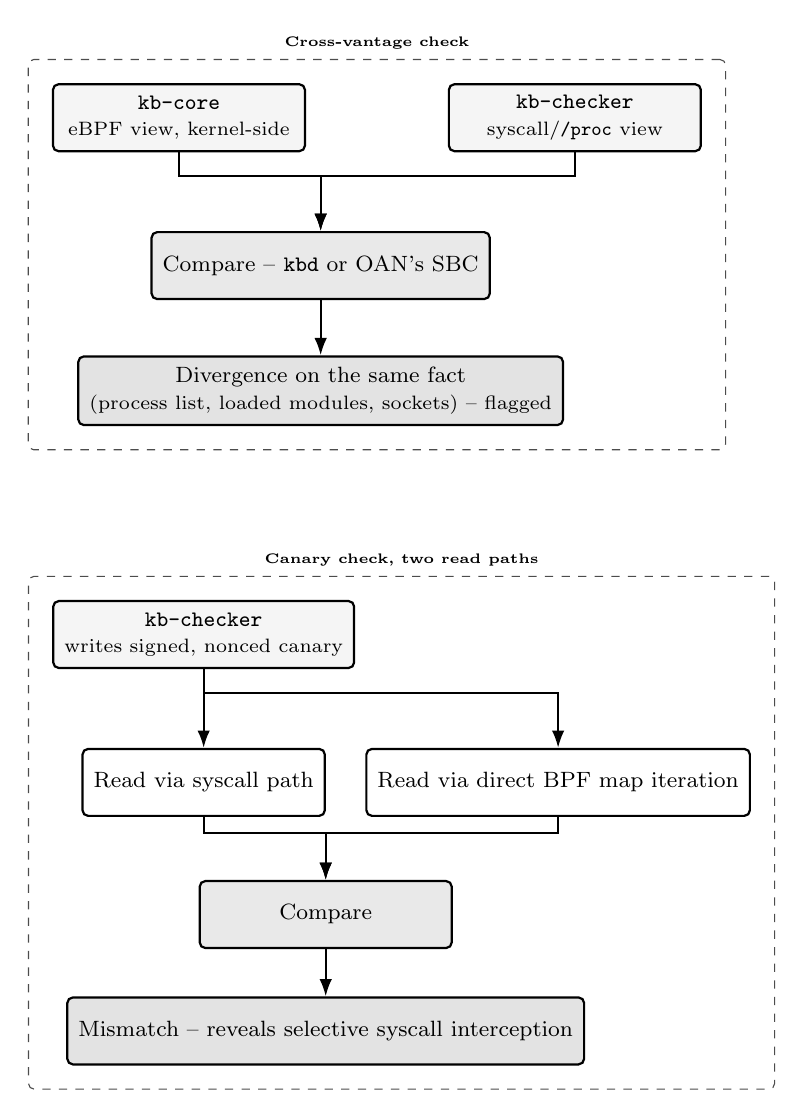
\begin{tikzpicture}[node distance=0.5cm and 0.9cm, font=\footnotesize]
  \node[hostblock, minimum width=3.2cm] (core) {\texttt{kb-core}\\\scriptsize eBPF view, kernel-side};
  \node[hostblock, right=1.8cm of core, minimum width=3.2cm] (kbc) {\texttt{kb-checker}\\\scriptsize syscall/\texttt{/proc} view};
  \node[oanblock, below=1.0cm of core, xshift=1.8cm, minimum width=3.6cm] (cmp) {Compare -- \texttt{kbd} or OAN's SBC};
  \draw[arr] (core.south) -- ++(0,-0.3) -| (cmp.north);
  \draw[arr] (kbc.south) -- ++(0,-0.3) -| (cmp.north);
  \node[block, below=0.7cm of cmp, minimum width=4.4cm, fill=gray!22] (flag) {Divergence on the same fact\\\scriptsize (process list, loaded modules, sockets) -- flagged};
  \draw[arr] (cmp) -- (flag);

  \node[groupbox, fit=(core)(kbc)(cmp)(flag), inner sep=0.3cm, label={[font=\tiny\bfseries]above:Cross-vantage check}] (panel1) {};

  \node[hostblock, below=1.9cm of panel1.south, minimum width=3.0cm, xshift=-2.2cm] (write) {\texttt{kb-checker}\\\scriptsize writes signed, nonced canary};
  \node[block, below=1.0cm of write, minimum width=2.6cm] (syscall) {Read via syscall path};
  \node[block, right=0.5cm of syscall, minimum width=2.6cm] (bpfread) {Read via direct BPF map iteration};
  \node[oanblock, below=0.8cm of syscall, xshift=1.55cm, minimum width=3.2cm] (cmp2) {Compare};
  \draw[arr] (write.south) -- ++(0,-0.3) -| (syscall.north);
  \draw[arr] (write.south) -- ++(0,-0.3) -| (bpfread.north);
  \draw[arr] (syscall.south) -- ++(0,-0.2) -| (cmp2.north);
  \draw[arr] (bpfread.south) -- ++(0,-0.2) -| (cmp2.north);
  \node[block, below=0.6cm of cmp2, minimum width=4.0cm, fill=gray!22] (flag2) {Mismatch -- reveals selective syscall interception};
  \draw[arr] (cmp2) -- (flag2);

  \node[groupbox, fit=(write)(syscall)(bpfread)(cmp2)(flag2), inner sep=0.3cm, label={[font=\tiny\bfseries]above:Canary check, two read paths}] (panel2) {};
\end{tikzpicture}
\figcap{Two comparisons, not two new components. \texttt{kb-core} and \texttt{kb-checker} already observe overlapping facts through different code paths -- the oldest rootkit-detection trick there is (raw vs.\ API view diffing)~\cite{hogland2005}. The canary variant targets the specific, most likely mechanism for lying to \texttt{kb-checker} without ever touching its binary: selective syscall interception.}
\label{fig:crosscheck}
\end{figure}

A rootkit that hooks the syscall table to lie to \texttt{kb-checker}
isn't automatically clever enough to also hide from an eBPF hook
watching the same fact from a different angle, and vice versa --
maintaining two consistent lies across two independent code paths is
strictly harder than maintaining one. Forwarding both views to a
single comparison point (\texttt{kbd}, or OAN's SBC over the OOB link)
costs nothing new to build; it's a comparison, not a component.

The canary variant sharpens this further: have \texttt{kb-checker}
periodically write a signed, nonced value into a BPF map, then read it
back two ways -- once through the normal syscall path, once through
direct BPF map iteration. A rootkit intercepting one path but not the
other reveals itself the moment the two answers disagree.

\subsection{Timing, Not Just Content}
\label{sec:timing}

Interception adds latency even when the forged output looks perfect --
intercepting a syscall, computing a plausible lie, and returning it
takes measurably longer than the kernel simply answering honestly.
Have \texttt{kb-checker} include its own attestation-generation time
in the signed payload, and have OAN's SBC track the \emph{distribution}
of that latency over the heartbeat interval, not any single sample.

\begin{plainbox}
A single slow heartbeat is noise -- a scheduler hiccup, a busy host.
A sustained \emph{shift in the shape} of that distribution is a side
channel: evidence that something now sits between \texttt{kb-checker}
and the kernel, independent of whether the reported content is
plausible at all.
\end{plainbox}

\subsection{Cross-Checking the Clock Itself}
\label{sec:clock-crosscheck}

OAN's SBC has its own independent wall clock by construction -- it is
a physically separate computer (\S\ref{sec:architecture}). Have
\texttt{kb-checker}'s attestation carry a monotonic counter and an
uptime figure, and have the SBC flag any inconsistency against the
real elapsed time since the last good heartbeat. This catches stealth
restarts, clock manipulation, or replay of an old, genuinely-valid
attestation -- cheap, and it uses nothing this design hasn't already
built.

\subsection{Classify the Failure, Don't Just Fence}
\label{sec:classify}

Fencing alone answers ``do something.'' It doesn't answer ``what
happened,'' and a report that just says \emph{OAN tripped} is barely
more useful than silence itself. The mitigations above don't need to
share one fencing trigger -- they need to feed one classification,
attached to the recovery event and surfaced through FMS
(\S\ref{sec:fms}).

\begin{center}
\renewcommand{\arraystretch}{1.45}
\small
\begin{tabular}{@{}p{2.9cm}p{4.6cm}p{5.5cm}@{}}
\toprule
\textbf{Bucket} & \textbf{Trigger} & \textbf{What it means} \\
\midrule
Silence & No heartbeat arrives before timeout (\S\ref{sec:heartbeat}) &
Process-level failure -- \texttt{kb-checker} killed, frozen, or
starved. Could be a crash; could be malicious. CPM
(\S\ref{sec:cpm-closed}) rules out KB's own pipeline as the cause. \\
Cryptographic failure & Heartbeat arrives, TPM signature or PCR-policy
check fails (\S\ref{sec:pcr-seal}) & High-confidence: measured-boot
state changed unexpectedly. The closest thing to a direct
rootkit/bootkit signature this design can produce. \\
Content implausibility & Signature valid, but canary, cross-vantage, or
timing invariants fail (\S\ref{sec:cross-consistency}--\S\ref{sec:clock-crosscheck}) &
\texttt{kb-checker} is alive and its key is intact, but something
beneath it is lying to it -- the confused-deputy case, specifically. \\
\bottomrule
\end{tabular}
\end{center}

That classification is the difference between ``OAN tripped'' and
``OAN tripped, category: cryptographic failure, consistent with an
unauthorized kernel module load.'' The second is something an operator
can actually act on.

The same judgment -- match the response to what's actually needed --
applies one layer down, at deployment time rather than incident time.
\texttt{kbd.service} and \texttt{kb-checker.service} keep only a
conservative baseline of systemd sandboxing directives~\cite{systemdexec}, not the fuller
capability-stripping and filesystem lockdown, because
\texttt{kb-checker}'s own Tampering Containment Protocol
(\S\ref{sec:recovery}) genuinely needs root and \texttt{CAP\_KILL},
\texttt{CAP\_NET\_ADMIN}, and bpffs-delete rights for its last-resort
lockdown -- a capability set gotten wrong there would fail silently
until the one moment it matters most. \texttt{kbagents},
\texttt{kbopd}, and \texttt{kbopt} get the full lockdown, safe to apply
precisely because none of them have anything resembling that need. The
same principle either way: hardening blind to what a component
actually has to do isn't hardening, it's a future outage waiting for
the day that need turns out to be real.

\subsection{Letting Weak Signals Accumulate Across the Fleet}
\label{sec:fleet-accumulate}

None of \S\ref{sec:cross-consistency}--\S\ref{sec:clock-crosscheck}
needs to be a hard trip-wire on its own -- a single near-miss on one
host might be noise. But \texttt{kb-aads} and FMS's cross-host
correlation (\S\ref{sec:fms}, already a stated if underdesigned
responsibility) can watch for the same \emph{pattern} of near-misses
showing up across multiple hosts around the same time. That is a much
stronger signal of deliberate, coordinated compromise than any one
host's isolated anomaly, and it costs nothing beyond forwarding
signals that already exist to a layer that already exists.

Concretely: Host 3 logs one clock-drift near-miss
(\S\ref{sec:clock-crosscheck}) at 02:14. Independently, Host 7 -- a
different Colony, connected to Host 3 only through FMS's signed
summaries, nothing lower-level -- logs a canary mismatch
(\S\ref{sec:cross-consistency}) at 02:15. Neither event alone crosses
that host's own fencing threshold; each looks, locally, like the
scheduler-hiccup or transient-noise case \S\ref{sec:clock-crosscheck}
already warns against over-reacting to. Correlated by FMS across the
fleet, the same ten-second window turns two individually-dismissible
shrugs into one incident: a coordinated action against multiple hosts,
timed together, that no single host's own local view could ever have
surfaced on its own.

Patterns worth correlating, not just individually counting:

\begin{itemize}
  \item \textbf{Classification-bucket clustering.} Several hosts
    landing in the same failure-classification bucket
    (\S\ref{sec:classify}) inside a short window, rather than the
    fleet's normal background rate of isolated, unrelated events.
  \item \textbf{Repeated interception fingerprints.} The same canary
    syscall path (\S\ref{sec:cross-consistency}) mismatching on more
    than one host -- consistent with one exploit technique deployed
    fleet-wide, not independent, unrelated compromises.
  \item \textbf{PCR-seal failures tied to a shared update batch.}
    Multiple hosts that recently received the \emph{same} patch or
    image failing PCR-sealed unseal around the same time points at a
    supply-chain question, not $N$ separate local incidents.
  \item \textbf{Clock anomalies clustering in wall-clock time.} Hosts
    have independent oscillators (\S\ref{sec:clock-crosscheck}); truly
    unrelated drift does not line up in time. When several do line up,
    that alignment is itself the signal.
\end{itemize}

One caveat carries over directly from \S\ref{sec:fms}'s Local Autonomy
Principle: this correlation layer is an enhancement, never a
dependency. Every host still evaluates and, if necessary, fences on
its own local signal with zero reliance on FMS being reachable --
fleet correlation adds context to an incident after the fact, it does
not gate whether any single host protects itself.

\subsection{What This Closes, and What Remains Open}

\begin{center}
\renewcommand{\arraystretch}{1.5}
\small
\begin{tabular}{@{}p{3.3cm}p{5.6cm}p{4.1cm}@{}}
\toprule
\textbf{Mitigation} & \textbf{Defends against} & \textbf{Residual gap} \\
\midrule
\texttt{kb-checker} in CPM's floor & KB's own containment pipeline
turning on its own watchdog & Nothing outside that pipeline \\
BPF map hardening (\S\ref{sec:bpf-map-hardening}) & In-kernel or
late-stage writes to CPM's own protected-list and containment maps &
Writes from userspace where a map isn't frozen; freeze is one-way and
only applied where nothing legitimate writes again \\
kb-core compiler hardening (\S\ref{sec:kbcore-hardening-confirmed}) &
Reliable memory-corruption exploitation of kb-core's own userspace
daemon -- the process managing CPM's maps and loading its eBPF
programs & Same residual as the row below \\
Key moved into the host's TPM & Passive key extraction from host RAM &
Active impersonation via the same signing API \\
PCR-sealed key usage (host TPM) & Impersonation by any attacker whose path to
Ring~0 loaded new code & Memory-corruption-only exploits; physical TPM
bus attacks; upstream firmware compromise \\
Memory-corruption narrowing (\S\ref{sec:memcorr-narrowing}) & Reliable
exploitation, code injection, stack hijack, and the measured-boot
bypass, layered together & A ROP/JOP or data-only exploit with no info
leak, evading every cross-check below \\
Cross-vantage \& canary checks & Selective syscall interception that
leaves kb-core's independent view untouched & A rootkit that fakes
\emph{both} views consistently \\
Timing \& clock cross-checks & Interception latency; stealth restarts;
attestation replay & Attacks with no measurable timing footprint \\
Failure classification & Turning a generic alarm into actionable
evidence & Doesn't itself detect anything new \\
systemd hardening split & Excess privilege on the operator/agent
services that don't need it & \texttt{kbd}/\texttt{kb-checker} keep
broad privilege by documented necessity -- hardening doesn't reach
their own attack surface \\
Fleet-level correlation & Coordinated, multi-host compromise below any
single host's hard threshold & A single, isolated, well-executed
compromise on one host \\
\bottomrule
\end{tabular}
\end{center}

\begin{notebox}[Status]
Most of this section is still design direction, at the same level of
maturity as the open questions already carried elsewhere in this
document -- concrete enough to build from, not yet a contract. Four
rows above are the exception, verified against the compiled output and
the actual diff, not just described: \texttt{kb-checker}'s CPM
protection, the BPF map hardening, kb-core's compiler hardening, and
the systemd hardening split are real and in the codebase today.
\S\ref{sec:pcr-seal} still needs a real design pass before it's
buildable: which PCR banks to bind to, the TPM2 policy-session
mechanics (\texttt{tpm2-tools}/\texttt{tpm2-tss},
\texttt{TPM2\_StartAuthSession} + \texttt{TPM2\_PolicyPCR}), and where
the re-sealing process lives operationally.
\end{notebox}

% =====================================================================
\section{How OAN Compares to Existing Approaches}
\label{sec:comparison}

OAN's shape -- an independent management processor, a hardware root of
trust, a physically separate network -- is not invented from nothing.
It follows patterns already proven at scale in adjacent fields, adapted
to Kernel Borderlands' specific job.

\begin{center}
\renewcommand{\arraystretch}{1.4}
\small
\begin{tabular}{@{}p{3.4cm}p{5.2cm}p{5.0cm}@{}}
\toprule
\textbf{Approach} & \textbf{What it shares with OAN} & \textbf{Where OAN differs} \\
\midrule
Enterprise BMC / IPMI~\cite{dmtfipmi} & Independent management processor, dedicated
network, works even if the main OS is down. & A BMC typically manages
one server for remote administration; OAN's primary purpose is
security attestation and fencing, with fleet management
(\S\ref{sec:fms}) built on top, not the other way around. \\
Hardware Security Module (HSM)~\cite{fips140} & Hardware-rooted key storage, tamper
resistance. & An HSM protects keys for applications to use; OAN's TPM
protects an attestation and fencing decision, not application
cryptography. \\
Academic out-of-band attestation research & Physically separate
verifier, independent of the host's own trust chain. & Most published
designs stop at detection; OAN adds a deterministic, host-independent
fencing action (\S\ref{sec:stm32}) as a first-class part of the
design, not a follow-on. \\
\bottomrule
\end{tabular}
\end{center}

The honest framing is that OAN combines ideas each of these fields has
already validated individually, applied together to one job: keeping
Kernel Borderlands' own trust anchor outside the reach of the exact
compromise it exists to catch.

% =====================================================================
\section{Frequently Asked Questions}
\label{sec:faq}

\begin{description}[leftmargin=1.2em, style=nextline, itemsep=0.7em]

\item[Can an attacker just unplug OAN?] \hfill \\
Physically, yes -- and that is a deliberate, visible action rather than
a silent software bypass. Because \texttt{kb-checker} expects a
heartbeat response on a fixed schedule (\S\ref{sec:heartbeat}), losing
the OOB link at all is itself the failure condition the fail-closed
policy is built to catch: no response, past timeout, triggers fencing
just as surely as an invalid response would.

\item[What stops someone from swapping OAN's SBC for a fake one that
always reports ``healthy''?] \hfill \\
The TPM. A forged SBC has no path to the sealed measurements the real
SBC's measured boot produced, so it cannot produce a verification the
TPM accepts (\S\ref{sec:tpm-relay}). This is exactly the property a
software-only check could not offer.

\item[Does OAN need to trust the network it runs on?] \hfill \\
The OOB Trust Plane, no -- it is physically isolated from any
production network by design (\S\ref{sec:planes}). The Fabric
Management Plane runs on ordinary networking, but it never carries
anything more sensitive than a signed summary that a compromised
network cannot forge (\S\ref{sec:fms}).

\item[What happens during a legitimate reboot or maintenance window?]
\hfill \\
An operator-initiated maintenance mode is expected to suppress fencing
for a bounded window, the same way any watchdog system needs a
sanctioned way to say ``this outage is expected.'' The heartbeat and
timeout mechanics themselves (\S\ref{sec:heartbeat}) are unchanged --
only whether the STM32 is allowed to act on a missed one.

\item[Why five hosts per chassis, and not, say, ten or twenty?] \hfill
\\ Blast radius, commodity part sizes, and the SBC's USB/GPIO budget
all independently point at the same number -- see
\S\ref{sec:scaling}'s ``Why Cap at Five Hosts'' for the full reasoning.

\item[Is OAN required to use Kernel Borderlands at all?] \hfill \\
No. Every host keeps full protection from \texttt{kb-core},
\texttt{kb-control-plane}, and \texttt{kb-checker} with no OAN present
at all. OAN adds a hardware trust anchor on top of an already-complete
software stack; it is a hardening layer, not a dependency.

\end{description}

% =====================================================================
\section{Positioning: What OAN Adds to Kernel Borderlands}

OAN extends Kernel Borderlands beyond a software-only runtime defense
framework by introducing a genuinely independent, hardware-assisted
trust layer. It gives the platform a verification domain that can
monitor host integrity, validate runtime attestation, coordinate
recovery, and perform last-resort fencing \emph{without ever depending
on the operating system it is protecting} -- closing the one gap a
same-host watchdog cannot structurally close on its own, and giving the
platform a foundation that scales from a single protected desk
(\S\ref{sec:architecture}) to a coordinated fleet (\S\ref{sec:scaling}
--\S\ref{sec:fms}) on the same trust model throughout.

% =====================================================================
\section{From Design to Deployment: The Build Roadmap}
\label{sec:roadmap}

Everything in this document describes one continuous architecture, but
it is built in three phases, each one a strict superset of the
hardware and guarantees the phase before it already established.

\begin{figure}[h!]
\centering
\resizebox{\linewidth}{!}{%
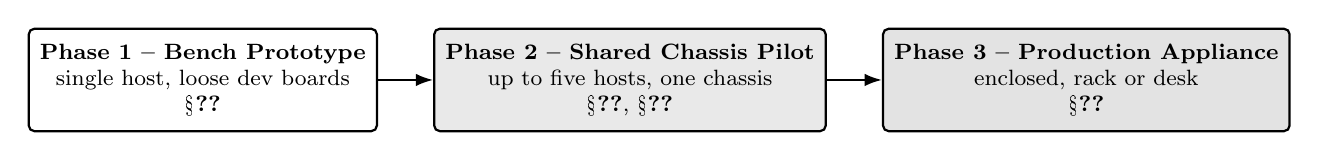
\begin{tikzpicture}[font=\scriptsize, node distance=0.55cm and 0.7cm]
  \node[block, minimum width=4.3cm, minimum height=1.3cm] (p1)
    {\textbf{Phase 1 -- Bench Prototype}\\single host, loose dev boards\\\S\ref{sec:bom}};
  \node[oanblock, right=of p1, minimum width=4.3cm, minimum height=1.3cm] (p2)
    {\textbf{Phase 2 -- Shared Chassis Pilot}\\up to five hosts, one chassis\\\S\ref{sec:scaling}, \S\ref{sec:walkthrough}};
  \node[block, right=of p2, minimum width=4.3cm, minimum height=1.3cm, fill=gray!22] (p3)
    {\textbf{Phase 3 -- Production Appliance}\\enclosed, rack or desk\\\S\ref{sec:properties}};

  \draw[arr] (p1) -- (p2);
  \draw[arr] (p2) -- (p3);
\end{tikzpicture}%
}
\figcap{Each phase reuses the same three-chip architecture (\S\ref{sec:three-chips}), the same TPM-rooted trust chain (\S\ref{sec:tpm-relay}), and the same recovery ladder (\S\ref{sec:recovery}). What changes across phases is packaging and host count, never the trust model.}
\label{fig:roadmap}
\end{figure}

\begin{center}
\renewcommand{\arraystretch}{1.35}
\small
\begin{tabular}{@{}p{2.4cm}p{6.3cm}p{5.6cm}@{}}
\toprule
\textbf{Phase} & \textbf{Goal} & \textbf{Exit condition} \\
\midrule
1. Bench Prototype & Prove the attestation heartbeat and fencing loop
end to end on one host, using loose commodity dev boards. & A full
heartbeat cycle (\S\ref{sec:heartbeat}) succeeds repeatedly, and a
deliberately broken link triggers the configured fencing policy
(\S\ref{sec:checklist}). \\
2. Shared Chassis Pilot & Validate the shared-hardware economics
(\S\ref{sec:bom}) and the fleet layer (\S\ref{sec:fms}) on a real,
multi-host chassis. & Five hosts registered with FMS, organized into
Families, reporting signed summaries continuously. \\
3. Production Appliance & Package the validated design into an
enclosed unit (\S\ref{sec:appliance-final}) suitable for a rack or a
shared desk, not a breadboard. & Front/rear panel design finalized;
internal layout addresses cooling and power regulation at sustained
load. \\
\bottomrule
\end{tabular}
\end{center}

\begin{plainbox}
No phase requires re-deciding anything about \emph{trust} -- only about
\emph{packaging and scale}. The TPM still seals the same two things
(\S\ref{sec:tpm-relay}), the STM32 still owns the relay alone
(\S\ref{sec:stm32}), and Stage 5 is still the last resort
(\S\ref{sec:recovery}) whether Phase 1's prototype is sitting on a
breadboard or Phase 3's appliance is bolted into a rack.
\end{plainbox}

% =====================================================================
\section{Glossary}

\begin{description}[leftmargin=3.2cm, style=nextline, itemsep=0.35em]
  \item[ASLR/KASLR] (Kernel) Address Space Layout Randomization --
    randomizes where code and data land in memory on every boot, so a
    memory-corruption bug that doesn't know where anything is usually
    just crashes rather than achieving reliable code
    execution~\cite{pax2003}.
  \item[Attestation] A signed statement from one component to another
    proving ``I am in the state I claim to be in,'' backed by
    cryptography rather than trust alone.
  \item[BMC] Baseboard Management Controller -- the enterprise-server
    equivalent of OAN's role: a small, independent management processor
    that keeps working even if the main OS is down~\cite{dmtfipmi}.
  \item[Confused Deputy] A program that is tricked into misusing its
    own legitimate authority on an attacker's behalf~\cite{hardy1988}
    -- the framing \S\ref{sec:whatif} uses for a \texttt{kb-checker}
    that is still running but has been fed false data.
  \item[eBPF] Extended Berkeley Packet Filter~\cite{mccanne1993,kernelebpf} -- the technology
    \texttt{kb-core} uses to observe kernel activity at Ring 0 without
    modifying the kernel itself.
  \item[Fencing] Physically isolating a compromised machine -- cutting
    its power, its reset line, or its network access -- so it can no
    longer act, whether or not its software cooperates.
  \item[Heartbeat] A signal sent at a fixed interval to prove a
    component is still alive and functioning correctly.
  \item[IMA] Integrity Measurement Architecture~\cite{sailer2004,kernelima}
    -- standard Linux, no new hardware -- extends a PCR every time a
    kernel module loads.
  \item[IWDG] Independent Watchdog -- a hardware timer peripheral on the
    STM32 that resets or triggers an action if not ``fed'' in time.
  \item[Kernel Ring 0] The most privileged execution level on a CPU,
    where the operating-system kernel itself runs.
  \item[KPTI] Kernel Page-Table Isolation -- closes Meltdown-class
    speculative-execution reads of kernel memory from
    userspace~\cite{lipp2018}, which indirectly closes one of the
    easiest ways to defeat KASLR before triggering a bug.
  \item[LKRG] Linux Kernel Runtime Guard~\cite{lkrg} -- an active,
    same-privilege-level kernel integrity monitor; see
    \S\ref{sec:lkrg-report-only} for why it belongs in report-only
    mode, not enforcement mode.
  \item[Measured Boot] Firmware, bootloader, kernel, and initrd each
    hash-measure the next stage before executing it, extending the
    result into TPM PCRs -- the chain \S\ref{sec:pcr-seal}'s
    PCR-sealing depends on.
  \item[OOB] Out-of-Band -- a communication channel that is physically
    or logically separate from a system's normal, in-band data path.
  \item[PCR] Platform Configuration Register~\cite{tcgtpm2,tcgpcclient}
    -- a TPM register that is only extendable, never directly
    writable, forming a one-way hash chain rooted at boot.
  \item[Root of Trust] The one component in a system that everything
    else's trust is ultimately built on -- if it is compromised, no
    higher-level check can be relied on.
  \item[Rootkit] Malware that hides its own presence, typically by
    subverting the kernel or a privileged process it runs
    inside~\cite{hogland2005}.
  \item[ROP/JOP] Return-Oriented / Jump-Oriented Programming -- exploit
    techniques that reuse already-legitimate, already-executable code
    instead of injecting new code, so
    W\textasciicircum X~\cite{deraadt2005} is silent on
    them~\cite{shacham2007,bletsch2011}.
  \item[TPM] Trusted Platform Module -- a dedicated hardware chip for
    secure key storage, measured boot, and integrity attestation.
  \item[Watchdog] A component whose job is to detect when something else
    has failed and to take a predefined recovery action.
  \item[W\textasciicircum X] Write XOR Execute -- a memory page is
    either writable or executable, never
    both~\cite{deraadt2005}, blocking the classic ``inject
    shellcode, jump to it'' technique but not ROP/JOP.
\end{description}

% =====================================================================
\section{Build Checklist}
\label{sec:checklist}

A practical, ordered checklist for a team building a first shared
chassis (\S\ref{sec:scaling}), grouped by the same stages as the
deployment walkthrough (\S\ref{sec:walkthrough}).

\subsection{Before Ordering Parts}

\begin{itemize}[label=$\square$]
  \item Confirm the host machine has a free USB or serial port, and a
    TPM header/SPI bus if the discrete TPM will sit on the host side of
    any wiring.
  \item Decide fail-open vs.\ fail-closed per host class
    (\S\ref{sec:tpm-relay}) before wiring, not after.
  \item Choose reference-cost or budget-cost parts (\S\ref{sec:bom}
    vs.\ \S\ref{sec:budget}) -- the discrete TPM and the STM32 split
    are never optional, at either budget.
  \item Decide how many hosts this first chassis will serve (1--5) --
    the shared parts are bought once regardless, so under-provisioning
    per-host parts is the only real risk of ordering too little.
\end{itemize}

\subsection{Assembling the Shared Chassis}

\begin{itemize}[label=$\square$]
  \item Flash the SBC's microSD with the base OS and the attestation
    engine.
  \item Wire the TPM module to the SBC and verify measured boot
    produces a stable, repeatable sealed measurement.
  \item Flash the ESP32 and confirm it can reach the dedicated OOB
    switch, and \emph{cannot} reach any production network segment.
  \item Connect the optional display and confirm it reflects SBC/STM32
    state (read-only, \S\ref{sec:tpm-relay}).
\end{itemize}

\subsection{Wiring the First Host}

\begin{itemize}[label=$\square$]
  \item Flash the STM32 channel with the deterministic watchdog
    firmware; confirm its IWDG fires correctly on a bench test
    \emph{before} wiring it to a real host's relay.
  \item Wire the relay to the host's power/reset header -- verify the
    NO/NC contacts match the intended fail-open/fail-closed policy for
    this host.
  \item Connect the dedicated OOB dongle, distinct from the host's main
    NIC.
  \item Install and start \texttt{kb-checker} on the host, and confirm
    a full heartbeat cycle (\S\ref{sec:heartbeat}, steps 1--4) succeeds
    repeatedly before trusting the link.
  \item Deliberately break the link (unplug the dongle) and confirm the
    configured failure policy actually fires within the expected
    timeout -- an untested failure path is not a working one.
\end{itemize}

\subsection{Scaling the Chassis}

\begin{itemize}[label=$\square$]
  \item Repeat ``Wiring the First Host'' for each additional host, up
    to the five-host cap (\S\ref{sec:scaling}).
  \item Register each new Node with FMS and assign it to a Family
    (\S\ref{sec:fms}).
  \item At the cap, provision a second independent chassis rather than
    extending this one (\S\ref{sec:scaling}'s blast-radius rationale).
\end{itemize}

\subsection{Hardening Against Boot-Time and Rootkit Compromise (Optional, \S\ref{sec:whatif})}

\begin{itemize}[label=$\square$]
  \item Confirm the \emph{host's own} TPM 2.0 is present and enabled in
    firmware (Intel PTT / AMD fTPM, or discrete) -- this is separate
    from OAN's own TPM and does the job described in
    \S\ref{sec:pcr-seal}, not the relay job in \S\ref{sec:tpm-relay}.
  \item Seal \texttt{kb-checker}'s OOB signing key to the host's own
    PCR values via \texttt{TPM2\_PolicyPCR}; verify the unseal succeeds
    on a clean boot and fails after a simulated PCR extend, using the
    PCR~16 sandbox walkthrough (\S\ref{sec:demo-env}) before touching
    PCRs~0--10 on a production host.
  \item Verify \texttt{kb-core}'s userspace binaries actually carry the
    compiler-hardening flags against the compiled output, not just the
    Makefile: \texttt{readelf} for PIE and full RELRO, \texttt{nm} for
    the stack-protector symbol (\S\ref{sec:kbcore-hardening-confirmed}).
  \item Enable Linux's \texttt{kernel\_lockdown} LSM; confirm
    \texttt{kexec\_load} is blocked and \texttt{kexec\_file\_load}
    only accepts images signed by a trusted key. Restrict
    \texttt{/dev/mem} and \texttt{/dev/kmem}
    (\texttt{CONFIG\_STRICT\_DEVMEM}).
  \item Decide whether to deploy LKRG for this host class. If yes, run
    it in logging/alert-only mode (\S\ref{sec:lkrg-report-only}) --
    never its process-kill/panic modes -- and fold its own presence
    into the measured baseline \emph{before} sealing PCRs, so it is
    expected at PCR-seal time rather than flagged as drift.
  \item Confirm the systemd hardening split from
    \texttt{boot\_sequence\_spec.md} is actually applied per unit --
    conservative baseline on \texttt{kbd.service}/\texttt{kb-checker.service},
    full lockdown on \texttt{kbagents.service}/\texttt{kbopd.service}/\texttt{kbopt.service}.
\end{itemize}

% =====================================================================
\section{Summary Cheat-Sheet}
\label{sec:cheatsheet}

A one-page recap of the facts a reader is most likely to need again
later, without re-reading the full document.

\begin{center}
\renewcommand{\arraystretch}{1.35}
\small
\begin{longtable}{@{}p{3.6cm}p{9.8cm}@{}}
\toprule
\textbf{What} & \textbf{Answer} \\
\midrule
\endhead
What OAN is & A physically separate hardware appliance that attests to
and can fence a Kernel Borderlands host, independent of that host's own
kernel. \\
What it talks to on the host & Only \texttt{kb-checker}, over a
dedicated out-of-band link (\S\ref{sec:architecture}). \\
Its three processors & SBC (brain), STM32 (spinal reflex), ESP32
(mouth) -- \S\ref{sec:three-chips}. \\
Its root of trust & A discrete TPM 2.0, sealing both OAN's own state
and the host's reported state (\S\ref{sec:tpm-relay}). \\
Its failure policy & Configurable; defaults to fail-closed
(\S\ref{sec:tpm-relay}). \\
Where it sits in recovery & Stage 5 of 5, strictly below
\texttt{kb-checker}'s existing software chain (\S\ref{sec:recovery}). \\
Reference deployment model & One shared chassis per up to five hosts
(\S\ref{sec:scaling}). \\
Fleet hierarchy & Fabric $\to$ Colony (one chassis) $\to$ Family
(purpose grouping) $\to$ Node (one host) -- \S\ref{sec:fms}. \\
Cost, one host & \$106--195 / INR 9,220--16,965 reference; \$54--76 /
INR 4,698--6,612 budget (\S\ref{sec:bom}, \S\ref{sec:budget}). \\
Cost, five hosts (one chassis) & \$234--383 / INR 20,360--33,320
reference; \$114--168 / INR 9,918--14,616 budget. \\
What is never cut, at any budget & The discrete TPM and the STM32
split (\S\ref{sec:budget}). \\
What FMS can and cannot weaken & Coordinates the fleet; never sits in
any single host's runtime security path (\S\ref{sec:autonomy}). \\
\bottomrule
\end{longtable}
\end{center}

% =====================================================================
\section{Appendix: Document Map}

This document is a plain-language synthesis. The full engineering
detail behind each section lives in the Kernel Borderlands
documentation tree:

\begin{center}
\renewcommand{\arraystretch}{1.6}
\small
\begin{tabular}{@{}p{4.6cm}@{\hspace{0.6cm}}l@{}}
\toprule
\textbf{Section here} & \textbf{Source documentation} \\
\midrule
Problem, philosophy, architecture, hardware, heartbeat, recovery ladder &
\path{docs/features/hardware-ext/} \newline \path{oan-hardware-appliance.md} \\[0.3em]
Fleet scaling, Fabric $\to$ Colony $\to$ Family $\to$ Node, FMS
responsibilities &
\path{docs/features/hardware-ext/oan-fms.md} \\[0.3em]
Budget build, cost-reduction levers &
\path{docs/features/hardware-ext/oan-cheap.md} \\[0.3em]
Boot/rootkit compromise resistance, PCR-sealing, this section's markdown twin &
\path{docs/features/hardware-ext/} \newline \path{oan-rootkit-resistance.md} \\[0.3em]
\texttt{kb-checker}'s existing software recovery chain &
\path{kb-checker/README.md} \\[0.3em]
Critical Process Module, ``fail closed toward protection'' &
\path{docs/features/CPM.md} \\[0.3em]
Critical Workload Protection &
\path{docs/features/CWP.md} \\[0.3em]
Socket topology, boot ordering &
\path{docs/architecture/boot\_sequence\_spec.md} \\
\bottomrule
\end{tabular}
\end{center}

% =====================================================================
\section{The Complete Picture: Full System Diagram}
\label{sec:fulldiagram}

One last, comprehensive view, folding every diagram in this document
into one picture. It is turned 90\textdegree\ on the page -- unlike
every other, upright figure in this document -- purely because its
content is wide: rotating it is what lets every layer, from the fleet
down to a single host's own internal stack, stay at a readable size
instead of being shrunk to fit a portrait column.

The complete picture, top to bottom: the Fleet layer (FMS coordinating
multiple Colonies), one Colony's shared OAN chassis, its per-host
STM32/relay channels, the protected hosts themselves, and one host's
own existing Kernel Borderlands software stack -- all five subsystems
(\texttt{kb-core}, \texttt{kb-control-plane}, \texttt{kb-op},
\texttt{kb-aads}, \texttt{kb-checker}) -- underneath it all.

Figure~\ref{fig:fulldiagram} (next page) packs a lot into one rotated
view. Read top to bottom, here is what every labeled box in it is:

\begin{center}
\renewcommand{\arraystretch}{1.35}
\small
\begin{tabular}{@{}p{3.6cm}p{10.6cm}@{}}
\toprule
\textbf{Component} & \textbf{Role in the diagram} \\
\midrule
Fabric \& FMS & Coordinates every Colony in the fleet (\S\ref{sec:fms}) -- non-security-critical, on its own Fabric Management Plane, never in a single host's runtime security path. \\
Other Colonies & The rest of the fleet -- each an independent, self-contained shared chassis exactly like the one drawn in full. \\
SBC (shared) & The chassis's attestation/policy engine -- ``the brain'' (\S\ref{sec:three-chips}). Runs the software that talks TPM and drives the fleet link. \\
ESP32 (shared) & ``The mouth'' -- management/comms only, kept out of the trust-critical path due to its larger, network-facing attack surface. \\
TPM (shared) & OAN's own root of trust (\S\ref{sec:tpm-relay}) -- seals OAN's own integrity and verifies what \texttt{kb-checker} reports. Distinct from any host's own TPM (\S\ref{sec:pcr-seal}). \\
Display (shared) & Optional, read-only reflection of SBC/STM32 state -- never a control surface. \\
STM32 ch.~1--5 & ``The spinal reflex'' -- one deterministic safety-controller channel per host, each running the heartbeat/fencing logic independent of the SBC's own Linux failure domain. \\
Relay & The physical fencing actuator each STM32 channel drives -- cuts a host's power or reset line on a fencing decision. \\
Host 1--5 & The protected machines themselves, each wired to its own STM32 channel and carrying its own dedicated OOB link (Figure~3). \\
\texttt{kb-core} & Ring-0 eBPF sensors on the host -- the deepest existing KB vantage point, and what the OOB Trust Plane ultimately corroborates. \\
\texttt{kb-control-plane} (\texttt{kbd}) & Ingests \texttt{kb-core}'s telemetry over \texttt{kbd.sock}, scores it, and pushes containment/control back down over the separate \texttt{kbct.sock}. \\
\texttt{kb-checker} & The existing software watchdog -- watches the rest of the stack independently, and is the one component that also feeds the OOB Trust Plane up to OAN's SBC (Figure~2). \\
\texttt{kb-op} & Operator interfaces -- \texttt{kb-tui}, \texttt{kb-dashboard}, \texttt{kbctl}, \texttt{kb-mcp} -- talking to \texttt{kbd} over gRPC/WebSockets. \\
\texttt{kb-aads} & The Python agent swarm, driven by the same \texttt{kbd} API as \texttt{kb-op}. \\
\bottomrule
\end{tabular}
\end{center}

\begin{sidewaysfigure}
\centering
\resizebox{!}{0.7\textwidth}{%
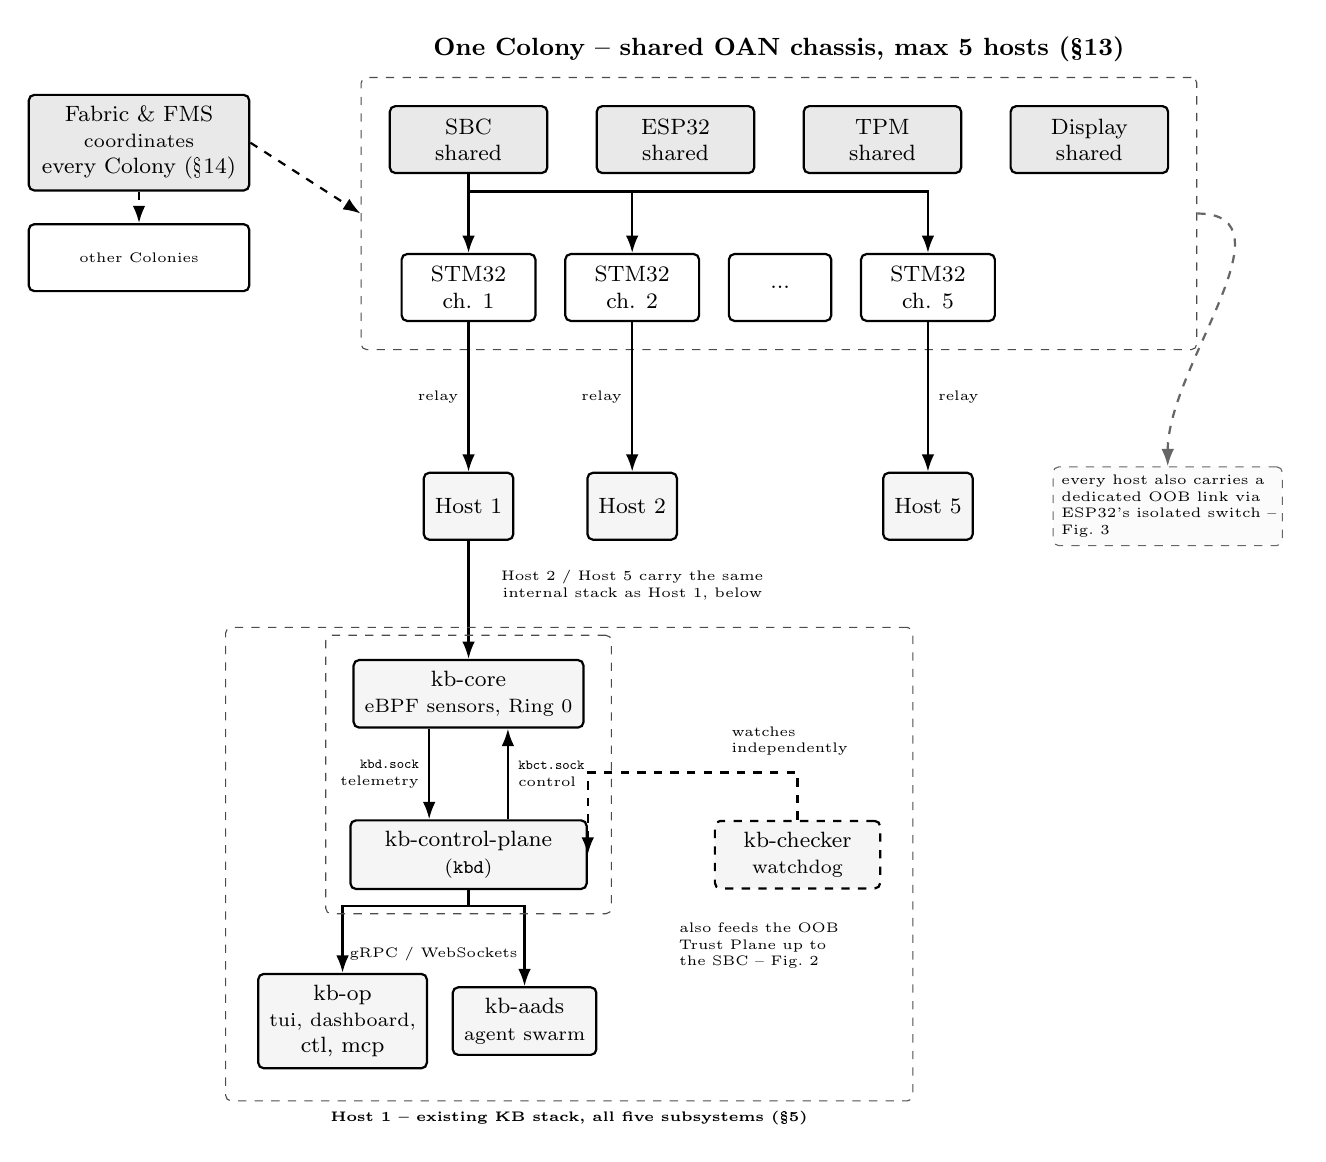
\begin{tikzpicture}[font=\scriptsize, node distance=0.5cm and 0.6cm]

  % ---- Shared chassis row ----
  \node[oanblock, minimum width=2.0cm] (sbc) {SBC\\shared};
  \node[oanblock, right=of sbc, minimum width=2.0cm] (esp) {ESP32\\shared};
  \node[oanblock, right=of esp, minimum width=2.0cm] (tpm) {TPM\\shared};
  \node[oanblock, right=of tpm, minimum width=2.0cm] (disp) {Display\\shared};

  % ---- STM32 channel row ----
  \node[block, below=1.0cm of sbc, minimum width=1.7cm] (c1) {STM32\\ch. 1};
  \node[block, right=0.35cm of c1, minimum width=1.7cm] (c2) {STM32\\ch. 2};
  \node[block, right=0.35cm of c2, minimum width=1.3cm] (c3) {...};
  \node[block, right=0.35cm of c3, minimum width=1.7cm] (c5) {STM32\\ch. 5};

  \draw[arr] (sbc.south) -- ++(0,-0.22) -| (c1.north);
  \draw[arr] (sbc.south) -- ++(0,-0.22) -| (c2.north);
  \draw[arr] (sbc.south) -- ++(0,-0.22) -| (c5.north);

  \node[groupbox, fit=(sbc)(esp)(tpm)(disp)(c1)(c2)(c3)(c5), inner sep=0.35cm] (chassis) {};
  \node[font=\small\bfseries] at ($(chassis.north)+(0,0.35)$) {One Colony -- shared OAN chassis, max 5 hosts (\S13)};

  % ---- Fleet layer, as a compact side branch off the chassis (reads on
  % the side, not stacked above -- keeps the tight dimension short) ----
  \node[oanblock, left=1.4cm of chassis, minimum width=2.8cm, yshift=0.9cm] (fabric)
    {Fabric \& FMS\\\scriptsize coordinates\\every Colony (\S14)};
  \draw[darr] (fabric.east) -- (chassis.west);
  \node[block, below=0.4cm of fabric, minimum width=2.8cm, font=\tiny, align=center] (othercol)
    {other Colonies};
  \draw[darr] (fabric.south) -- (othercol.north);

  % ---- Host row ----
  \node[hostblock, below=1.9cm of c1] (h1) {Host 1};
  \node[hostblock, below=1.9cm of c2] (h2) {Host 2};
  \node[hostblock, below=1.9cm of c5] (h5) {Host 5};

  \draw[arr] (c1.south) -- node[left, font=\tiny]{relay} (h1.north);
  \draw[arr] (c2.south) -- node[left, font=\tiny]{relay} (h2.north);
  \draw[arr] (c5.south) -- node[right, font=\tiny]{relay} (h5.north);

  \node[draw=black!60, dashed, rounded corners=2pt, fill=gray!3, right=1.0cm of h5,
    font=\tiny, align=left, text width=2.7cm, inner sep=3pt] (oobnote)
    {every host also carries a dedicated OOB link via ESP32's isolated switch -- Fig.~3};
  \draw[darr, black!60] (chassis.east) to[out=0, in=90] (oobnote.north);

  \node[font=\tiny, align=center, below=0.25cm of h2, text width=3.6cm] (samenote)
    {Host 2 / Host 5 carry the same internal stack as Host 1, below};

  % ---- Host 1's own internal software stack -- all five KB subsystems ----
  \node[hostblock, below=1.5cm of h1, minimum width=2.4cm] (core) {kb-core\\\scriptsize eBPF sensors, Ring 0};
  \node[hostblock, below=1.15cm of core, minimum width=3.0cm] (cp) {kb-control-plane\\\scriptsize (\texttt{kbd})};

  \draw[arr] (h1.south) -- ++(0,-0.25) -| (core.north);
  \draw[arr] ($(core.south)+(-0.5,0)$) -- ($(cp.north)+(-0.5,0)$)
    node[midway, left, font=\tiny, align=right]{\texttt{kbd.sock}\\telemetry};
  \draw[arr] ($(cp.north)+(0.5,0)$) -- ($(core.south)+(0.5,0)$)
    node[midway, right, font=\tiny, align=left]{\texttt{kbct.sock}\\control};

  \node[hostblock, below=1.05cm of cp, minimum width=2.1cm, xshift=-1.6cm] (op) {kb-op\\\scriptsize tui, dashboard,\\ctl, mcp};
  \node[hostblock, right=0.3cm of op, minimum width=1.8cm] (aads) {kb-aads\\\scriptsize agent swarm};

  \draw[arr] (cp.south) -- ++(0,-0.2) -| (op.north);
  \draw[arr] (cp.south) -- ++(0,-0.2) -| (aads.north);
  \node[font=\tiny] at ($(op.north)!0.5!(aads.north)+(0,0.32)$) {gRPC / WebSockets};

  \node[groupbox, fit=(core)(cp), inner sep=0.3cm] (watched) {};

  \node[hostblock, dashed, right=1.6cm of cp, minimum width=2.1cm] (kbc) {kb-checker\\\scriptsize watchdog};
  \draw[darr] (kbc.north) -- ++(0,0.6) -| (cp.east);
  \node[font=\tiny, align=left] at ($(kbc.north)+(-0.1,1.0)$) {watches\\independently};

  \node[groupbox, fit=(core)(cp)(op)(aads)(kbc), inner sep=0.4cm,
    label={[font=\tiny\bfseries]below:Host 1 -- existing KB stack, all five subsystems (\S5)}] (hoststack) {};

  \node[font=\tiny, align=left, below=0.3cm of kbc, text width=3.0cm]
    {also feeds the OOB\\Trust Plane up to\\the SBC -- Fig.~2};

\end{tikzpicture}%
}
\caption{The complete picture, top to bottom.}
\label{fig:fulldiagram}
\end{sidewaysfigure}
\FloatBarrier

% =====================================================================
\section{References}
\label{sec:references}

\renewcommand{\refname}{}
\begin{thebibliography}{99}

\bibitem{repo} Kernel Borderlands project repository. \url{https://github.com/pardhuvarmax/kernel-borderlands/tree/main}.

\bibitem{hardy1988} N.~Hardy, ``The Confused Deputy: (or why capabilities might have been invented),'' \emph{ACM SIGOPS Operating Systems Review}, vol.~22, no.~4, pp.~36--38, 1988.

\bibitem{bishop1996} M.~Bishop and M.~Dilger, ``Checking for Race Conditions in File Accesses,'' \emph{Computing Systems}, vol.~9, no.~2, pp.~131--152, 1996.

\bibitem{tcgtpm2} Trusted Computing Group, \emph{Trusted Platform Module Library Specification, Family ``2.0''}. \url{https://trustedcomputinggroup.org}.

\bibitem{tcgpcclient} Trusted Computing Group, \emph{PC Client Platform Firmware Profile Specification}. \url{https://trustedcomputinggroup.org}.

\bibitem{sailer2004} R.~Sailer, X.~Zhang, T.~Jaeger, and L.~van~Doorn, ``Design and Implementation of a TCG-based Integrity Measurement Architecture,'' in \emph{Proc.\ 13th USENIX Security Symposium}, 2004.

\bibitem{kernelima} \emph{Integrity Measurement Architecture (IMA)}, The Linux Kernel Documentation. \url{https://www.kernel.org/doc/}.

\bibitem{kernellockdown} \emph{Kernel Lockdown LSM}, The Linux Kernel Documentation. \url{https://www.kernel.org/doc/}.

\bibitem{kernelmodsig} \emph{Kernel Module Signing Facility}, The Linux Kernel Documentation. \url{https://www.kernel.org/doc/}.

\bibitem{pax2003} PaX Team, \emph{PaX Address Space Layout Randomization (ASLR)}, design document, 2003.

\bibitem{cowan1998} C.~Cowan, C.~Pu, D.~Maier, H.~Hinton, J.~Walpole, P.~Bakke, S.~Beattie, A.~Grier, P.~Wagle, and Q.~Zhang, ``StackGuard: Automatic Adaptive Detection and Prevention of Buffer-Overflow Attacks,'' in \emph{Proc.\ 7th USENIX Security Symposium}, 1998.

\bibitem{intelcet} Intel Corporation, \emph{Control-flow Enforcement Technology Specification}.

\bibitem{deraadt2005} T.~de~Raadt, ``Exploit Mitigation Techniques,'' OpenBSD Project (W\textasciicircum X design), 2005.

\bibitem{solardesigner1997} Solar Designer, ``Getting around non-executable stack (and fix),'' Bugtraq mailing list, 1997.

\bibitem{shacham2007} H.~Shacham, ``The Geometry of Innocent Flesh on the Bone: Return-into-libc without Function Calls (on the x86),'' in \emph{Proc.\ ACM Conference on Computer and Communications Security (CCS)}, 2007.

\bibitem{bletsch2011} T.~Bletsch, X.~Jiang, V.~Freeh, and Z.~Liang, ``Jump-Oriented Programming: A New Class of Code-Reuse Attack,'' in \emph{Proc.\ 6th ACM Symposium on Information, Computer and Communications Security (ASIACCS)}, 2011.

\bibitem{lipp2018} M.~Lipp, M.~Schwarz, D.~Gruss, T.~Prescher, W.~Haas, A.~Fogh, J.~Horn, S.~Mangard, P.~Kocher, D.~Genkin, Y.~Yarom, and M.~Hamburg, ``Meltdown: Reading Kernel Memory from User Space,'' in \emph{Proc.\ 27th USENIX Security Symposium}, 2018.

\bibitem{gruss2017} D.~Gruss, M.~Lipp, M.~Schwarz, R.~Fellner, C.~Maurice, and S.~Mangard, ``KASLR is Dead: Long Live KASLR,'' in \emph{Proc.\ International Symposium on Engineering Secure Software and Systems (ESSoS)}, 2017.

\bibitem{lkrg} Openwall Project, \emph{Linux Kernel Runtime Guard (LKRG)}. \url{https://github.com/openwall/lkrg}.

\bibitem{intelptt} Intel Corporation, \emph{Platform Trust Technology (PTT)}, part of Intel Trusted Execution Technology documentation.

\bibitem{amdftpm} AMD, \emph{AMD Secure Technology --- Firmware TPM (fTPM)} documentation.

\bibitem{dmtfipmi} Distributed Management Task Force / Intel, \emph{Intelligent Platform Management Interface (IPMI) Specification}. \url{https://www.dmtf.org}.

\bibitem{fips140} National Institute of Standards and Technology, \emph{FIPS 140-3: Security Requirements for Cryptographic Modules}, 2019.

\bibitem{nist800155} National Institute of Standards and Technology, \emph{NIST SP 800-155: BIOS Integrity Measurement Guidelines} (draft).

\bibitem{uefispec} UEFI Forum, \emph{Unified Extensible Firmware Interface (UEFI) Specification} (Secure Boot). \url{https://uefi.org}.

\bibitem{mccanne1993} S.~McCanne and V.~Jacobson, ``The BSD Packet Filter: A New Architecture for User-level Packet Capture,'' in \emph{Proc.\ USENIX Winter Conference}, 1993.

\bibitem{kernelebpf} \emph{BPF and XDP Reference Guide}, The Linux Kernel Documentation. \url{https://www.kernel.org/doc/}.

\bibitem{tpm2software} tpm2-software Community, \emph{tpm2-tools} and \emph{tpm2-tss}. \url{https://github.com/tpm2-software}.

\bibitem{systemdexec} \emph{systemd.exec(5)} --- sandboxing directives (\texttt{NoNewPrivileges=}, \texttt{ProtectSystem=}, \texttt{CapabilityBoundingSet=}). \url{https://systemd.io}.

\bibitem{hogland2005} G.~Hoglund and J.~Butler, \emph{Rootkits: Subverting the Windows Kernel}. Addison-Wesley, 2005.

\bibitem{swtpm} Stefan Berger et al., \emph{swtpm --- TPM Emulator for QEMU/libvirt}. \url{https://github.com/stefanberger/swtpm}.

\bibitem{tcgpcr} Trusted Computing Group, \emph{TCG PC Client Platform TPM Profile (PTP) Specification} --- PCR index assignment (including the reserved/resettable ``debug'' PCRs used in \S\ref{sec:demo-env}).

\end{thebibliography}

\clearpage
\thispagestyle{empty}
\begin{center}
\vspace*{\fill}

{\small\textls[280]{KERNEL BORDERLANDS}}

\vspace{1.4cm}

{\fontsize{22}{26}\selectfont\bfseries Thank You}

\vspace{0.6em}

{\normalsize for reading through the Out-of-Band Attestation Node design}

\vspace{1.8cm}

{\small \scshape Team Kernel Borderlands}

\vspace{0.9em}

{\small \url{https://github.com/pardhuvarmax/kernel-borderlands}}

\vspace*{\fill}
\end{center}

\end{document}
